\documentclass[conference,10pt]{IEEEtran}
\IEEEoverridecommandlockouts
\usepackage[utf8]{inputenc}
\usepackage[T1]{fontenc}
\usepackage{amsmath,amssymb}
\usepackage{graphicx}
\usepackage{booktabs}
\usepackage{array}
\usepackage{cite}
\usepackage{url}
\usepackage{xcolor}
\usepackage{tikz}
\usepackage{pgfplots}
\pgfplotsset{compat=1.16}
\usetikzlibrary{arrows.meta,positioning,shapes.geometric,fit,calc,backgrounds}
\graphicspath{{../figures/}{./}}
\newcommand{\code}[1]{\texttt{\small\detokenize{#1}}}
\newcommand{\codes}[1]{\texttt{\detokenize{#1}}}
% Evidence classes
\newcommand{\evM}{\textsc{[measured]}}
\newcommand{\evO}{\textsc{[observed]}}
\newcommand{\evE}{\textsc{[exploratory]}}
\newcommand{\evU}{\textsc{[unresolved]}}
\newcommand{\evP}{\textsc{[proposed]}}
% One visual language for every diagram
\definecolor{cdata}{HTML}{1F4E79}
\definecolor{cctl}{HTML}{B45F06}
\definecolor{chum}{HTML}{A61C1C}
\definecolor{fhw}{HTML}{E8EEF4}
\definecolor{fproc}{HTML}{F4F4F4}
\definecolor{fdec}{HTML}{FFF4D6}
\definecolor{fstore}{HTML}{E6F2E6}
\definecolor{fext}{HTML}{F3E8F5}
\definecolor{fend}{HTML}{FBE4E4}
\tikzset{
  every picture/.append style={font=\scriptsize,>={Stealth[length=1.6mm]}},
  box/.style={draw,rounded corners=1pt,fill=fproc,align=center,inner sep=2pt,minimum height=5mm},
  hw/.style={box,fill=fhw},
  store/.style={box,fill=fstore},
  ext/.style={box,fill=fext,dashed},
  term/.style={box,fill=fend},
  dec/.style={draw,fill=fdec,align=center,inner sep=2pt,minimum height=5mm,rounded corners=5pt},
  group/.style={draw,gray,rounded corners=2pt,inner sep=4pt},
  grouplabel/.style={font=\scriptsize\bfseries,gray!40!black},
  d/.style={->,cdata,semithick},
  c/.style={->,cctl,semithick,dashed},
  h/.style={->,chum,semithick,densely dotted},
  yes/.style={midway,font=\tiny,fill=white,inner sep=0.5pt},
  panel/.style={font=\footnotesize\bfseries}
}

\begin{document}
\title{Third Eye: A Phone-Based Referee for Physical Jenga Using LiDAR Depth, Fiducial Pose and Compiled Rulebooks}
% CONFIRM BEFORE SUBMISSION: exact department or programme. The school below comes from CS3235_paper.tex.
\author{\IEEEauthorblockN{Aadit Pani, Megh Mavani, Mitul K M}
\IEEEauthorblockA{School of Computer Science and Engineering, RV University, Bengaluru, India}}
\maketitle

\begin{abstract}
Third Eye watches a physical Jenga game with an iPhone (LiDAR) and an optional Android phone, draws which blocks may be pulled, names the pulled block, and flags a collapse. This paper is an engineering case study of the system as built, including what did not work. It describes the implementation from the code, separates offline evaluation from live behaviour, and labels every result by the kind of evidence behind it. In an offline evaluation of the deployed scoring code, with the server's unweighted camera mean, the pulled layer was exact on 25 of 32 labelled pulls from 11 games (78\,\%; Wilson 95\,\% interval 61--89\,\%; the earlier 31-pull snapshot gave 24/31). These labels are optimistic because a confident, uncorrected answer counts as correct. Two negative results stand out: a LiDAR box fit did not beat markers alone on an edge-strength proxy for overlay placement (2.95 versus 3.07), and a simple percentile beat the fit on real, hand-free height frames (98\,\% versus 88\,\% exact layer). The current collapse detector caught the one real fall in three replayed games with no false alarm, which is very weak evidence. iPhone-versus-Android comparisons reverse between label sets and remain unresolved. Nothing here is held out, the private recordings cannot be published, and end-to-end latency and millimetre overlay error were not measured.
\end{abstract}
\begin{IEEEkeywords}
Jenga, LiDAR, ArUco, pose estimation, change detection, human-in-the-loop, negative results, case study
\end{IEEEkeywords}

\section{Introduction}
Refereeing a physical game needs the state of the pieces and a rulebook. For Jenga, the state is a stack of $L$ layers of three blocks, and the rules say which block may be taken and when the game has ended. Doing this with consumer phones is hard for a concrete reason: layers are 15\,mm tall, while published evaluations put phone LiDAR at about $\pm$1\,cm on objects larger than 10\,cm~\cite{luetzenburg2021}. The sensor cannot simply be read off.

Third Eye combines a fixed marker board, colour images, LiDAR depth, an explicit balance model and the player's confirmation. We make no claim of a new detector or tracker. The contribution is a detailed account of an integrated system and an honest evaluation of it, including approaches that did not earn their place. We ask:
\begin{itemize}
\item \textbf{RQ1.} What frame rates and data volumes does the phone rig sustain, and what bounds them?
\item \textbf{RQ2.} Does the LiDAR box fit improve overlay placement or height estimation over simpler baselines?
\item \textbf{RQ3.} How well does the deployed finder's scoring name the pulled layer offline, and what can be said about each camera?
\item \textbf{RQ4.} What evidence supports the current collapse detector?
\item \textbf{RQ5.} Where does the system depend on the human, and how does that limit what the evaluation can show?
\end{itemize}

Section~\ref{sec:related} reviews related work and Section~\ref{sec:problem} states the problem. Section~\ref{sec:design} describes the implementation. Section~\ref{sec:method} sets out the evaluation method and provenance of each result. Sections~\ref{sec:quant} and~\ref{sec:qual} report quantitative and qualitative findings, Section~\ref{sec:discussion} connects them, and Section~\ref{sec:threats} addresses threats to validity.

\section{Related Work}\label{sec:related}
\textbf{Jenga in robotics.} Fazeli et al.\ model Jenga with a temporal hierarchical Bayesian process and teach a robot to play by fusing force and vision, comparing against three baselines~\cite{fazeli2019}. Their problem is manipulation; ours is observing a human game with no force channel.

\textbf{Game-state recognition.} Wölflein and Arandjelović recover a chess position from one image using board localisation and two neural networks trained on a synthetic dataset, reporting 0.23\,\% per-square error on their test set~\cite{wolflein2021}. Chess pieces are visible from above and a position is a single picture. A Jenga pull changes a few square centimetres on a repeating structure, so we compare calibrated before-and-after views instead of classifying a state. Our searches did not find a published physical-Jenga referee; that is a limit of our search, not evidence that none exists.

\textbf{Procedural activity and mistakes.} Assembly101 offers 4321 multi-view videos (513\,h, 53 participants) of toy assembly with a mistake-detection task~\cite{sener2022}. Ding et al.\ build spatial and temporal beliefs as logic-like rules on that dataset and report 70.6\,\% recall on ordering mistakes~\cite{ding2023}. Their rules are learned from observation; ours are stated, and legality comes from an explicit balance model. Augmented-reality guidance for assembly is surveyed in~\cite{wang2016}.

\textbf{Fiducials, pose and edges.} We use ArUco markers~\cite{garrido2014}, IPPE~\cite{collins2014} and a calibrated board solved by bundle adjustment~\cite{triggs2000}, with lens calibration following Zhang~\cite{zhang2000}. Edge snapping is related to CAD-model edge tracking~\cite{drummond2002}, though it is a small one-shot search rather than a frame-rate tracker.

\textbf{Phone depth.} Beyond~\cite{luetzenburg2021}, Huang et al.\ describe iPhone LiDAR as noisy and low in resolution (256$\times$192) for object pose estimation~\cite{huang2023}. Dense fusion~\cite{newcombe2011} was tried early in this project and superseded, because ARKit's mesh triangles of about 30\,mm (project notes) cannot resolve 15\,mm layers.

\textbf{Robust fitting and change detection.} The fit uses Geman--McClure weights and a shrinking scale, connected to robust estimation through~\cite{black1996}. Yang et al.\ apply graduated non-convexity to this cost with a decreasing control parameter~\cite{yang2020}; our schedule resembles this but is not their method. Our finder falls within image change detection, surveyed in~\cite{radke2005}, and uses phase correlation~\cite{kuglin1975} to discount small shifts.

\textbf{Confidence and the human.} Rejecting uncertain decisions has a long history~\cite{chow1970}. Guo et al.\ define calibration as agreement between confidence and accuracy~\cite{guo2017}, a standard our small tier table cannot be shown to meet. Bondi et al.\ found in a 198-participant study that showing a model's prediction lowered human accuracy (57.8\,\% versus 60.2\,\%)~\cite{bondi2022}. That finding motivates a hypothesis below about our Yes/No prompt.

\textbf{Rules from text.} Mensfelt et al.\ translate game descriptions into logic programs with 100\,\% syntactic but 76.5\,\% semantic correctness~\cite{mensfelt2025}, a useful warning that a program passing validation need not mean what the text meant. The upstream Third Eye rule compiler faces the same risk.

\begin{table*}[!t]
\caption{Comparison with related work. Values are those we could verify; no performance comparison is implied because tasks and data differ.}\label{tab:related}
\centering\footnotesize
\begin{tabular}{@{}p{2.3cm}p{3.2cm}p{3.1cm}p{2.4cm}p{5.6cm}@{}}
\toprule
Work & Input & Task & Explicit rules & Reported evaluation \\
\midrule
Fazeli et al.~\cite{fazeli2019} & Force and vision, robot & Learn to extract blocks & Learned model & Three baselines, real game \\
Wölflein et al.~\cite{wolflein2021} & One RGB image & Chess state & Not applicable & 0.23\,\% per-square error, synthetic test set \\
Sener et al.~\cite{sener2022} & Multi-view video & Recognition, mistakes & None & 4321 videos, 53 participants \\
Ding et al.~\cite{ding2023} & Assembly101 labels & Ordering mistakes & Inferred beliefs & Mistake recall 70.6\,\% \\
\textbf{Third Eye} & Phone RGB, LiDAR, ArUco board, player input & Pull layer, legality, collapse & Balance model; upstream compiled specs & 25/32 exact offline, optimistic labels; one real fall \\
\bottomrule
\end{tabular}
\end{table*}

\section{Problem Formulation}\label{sec:problem}
A tower has $L$ layers with slots $s\in\{0,1,2\}$ and occupancy $o_{\ell s}\in\{0,1\}$. Blocks are 25$\times$75$\times$15\,mm. A move removes $(\ell,s)$ and normally returns the block to the top. Given images $I^c_t$ from cameras $c$, iPhone depth $D_t$ and the player's MARK tap, the referee outputs (a) the pulled block, (b) for every standing block whether it may be pulled, and (c) a game-over signal. The system is advisory and keeps a player in the loop. Placements are not observed: they are modelled by a flag (default on) that puts each pulled block on top.

\section{System Design}\label{sec:design}
This section describes the code at the commit under study. Table~\ref{tab:constants} collects the constants used below with their locations.

\subsection{Architecture}
Fig.~\ref{fig:arch}(a) shows the deployed system. Two capture apps post frames to a single-process Python server, which keeps the ledger of pulls and sends the browser raw pictures plus a short list of overlay shapes. Aadit Pani's separate Third Eye repository supplies the web interface, a rule checker, the rule compiler and an LLM explanation panel; it reaches the game server through a fixed allow-list proxy and follows confirmed pulls. Fig.~\ref{fig:arch}(b) shows which modules are live. The earlier per-slot tracker and mesh experiments remain in the repository but are not in the deployed path.

\begin{figure*}[!t]\centering
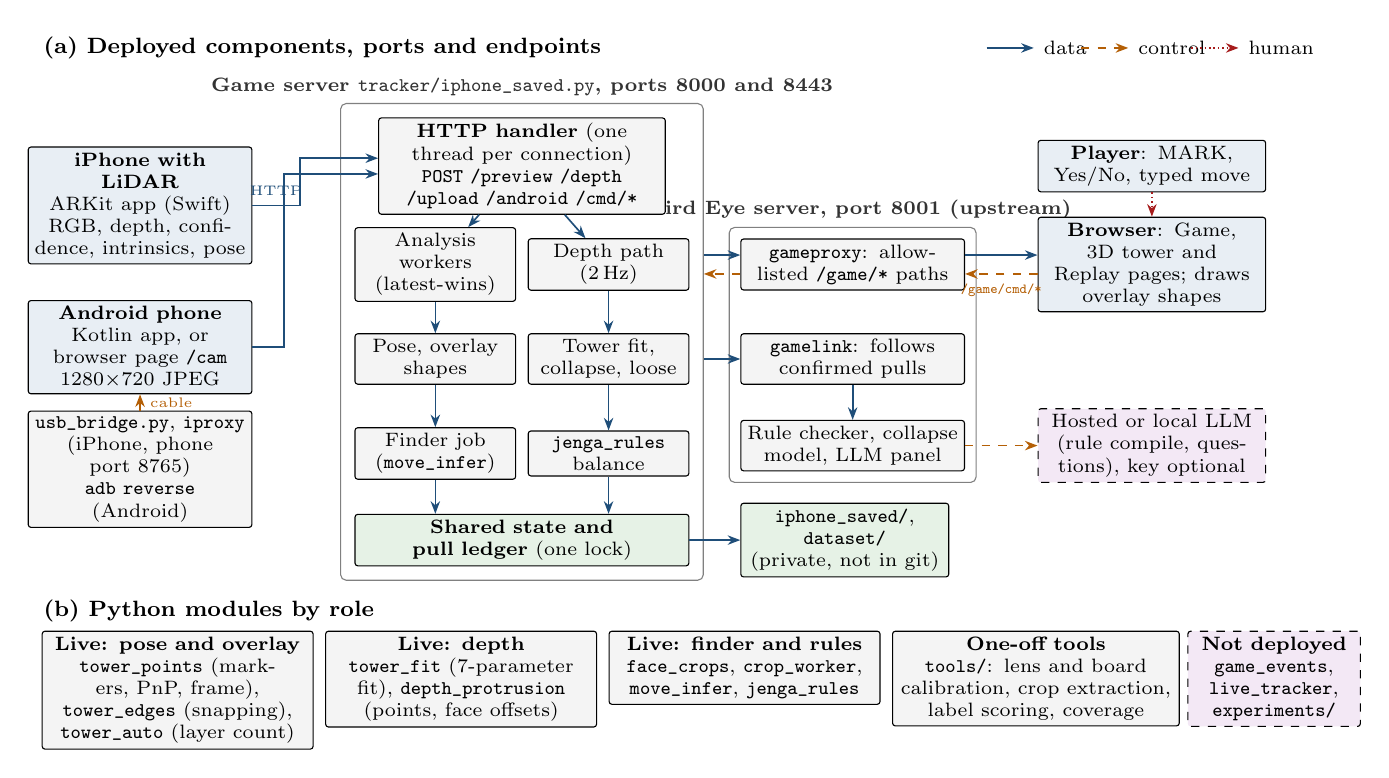
\begin{tikzpicture}[x=1cm,y=1cm]
\node[panel,anchor=west] at (-0.2,6.7) {(a) Deployed components, ports and endpoints};
% phones
\node[hw,text width=2.7cm] (ip) at (1.15,4.7) {\textbf{iPhone with LiDAR}\\ARKit app (Swift)\\RGB, depth, confidence, intrinsics, pose};
\node[hw,text width=2.7cm] (an) at (1.15,2.9) {\textbf{Android phone}\\Kotlin app, or browser page \codes{/cam}\\1280$\times$720 JPEG};
\node[box,text width=2.7cm] (br) at (1.15,1.35) {\codes{usb_bridge.py}, \codes{iproxy}\\(iPhone, phone port 8765)\\\codes{adb reverse} (Android)};
% server
\node[box,text width=3.5cm] (h) at (6.0,5.2) {\textbf{HTTP handler} (one thread per connection)\\ \codes{POST /preview /depth /upload /android /cmd/*}};
\node[box,text width=1.9cm] (w) at (4.9,3.95) {Analysis workers (latest-wins)};
\node[box,text width=1.9cm] (dp) at (7.1,3.95) {Depth path (2\,Hz)};
\node[box,text width=1.9cm] (po) at (4.9,2.75) {Pose, overlay shapes};
\node[box,text width=1.9cm] (co) at (7.1,2.75) {Tower fit, collapse, loose};
\node[box,text width=1.9cm] (fi) at (4.9,1.55) {Finder job (\codes{move_infer})};
\node[box,text width=1.9cm] (ru) at (7.1,1.55) {\codes{jenga_rules} balance};
\node[store,text width=4.1cm] (st) at (6.0,0.45) {\textbf{Shared state and pull ledger} (one lock)};
\begin{scope}[on background layer]
\node[group,fit=(h)(w)(dp)(po)(co)(fi)(ru)(st),inner sep=5pt,label={[grouplabel,anchor=south,yshift=-1pt]north:Game server \codes{tracker/iphone_saved.py}, ports 8000 and 8443}] (gs) {};
\end{scope}
% disk
\node[store,text width=2.5cm] (disk) at (10.1,0.45) {\codes{iphone_saved/}, \codes{dataset/}\\(private, not in git)};
% third eye
\node[box,text width=2.7cm] (px) at (10.2,3.95) {\codes{gameproxy}: allow-listed \codes{/game/*} paths};
\node[box,text width=2.7cm] (gl) at (10.2,2.75) {\codes{gamelink}: follows confirmed pulls};
\node[box,text width=2.7cm] (te) at (10.2,1.65) {Rule checker, collapse model, LLM panel};
\begin{scope}[on background layer]
\node[group,fit=(px)(gl)(te),label={[grouplabel,anchor=south,yshift=-1pt]north:Third Eye server, port 8001 (upstream)}] (ts) {};
\end{scope}
\node[hw,text width=2.75cm] (ui) at (14.0,3.95) {\textbf{Browser}: Game, 3D tower and Replay pages; draws overlay shapes};
\node[ext,text width=2.75cm] (llm) at (14.0,1.65) {Hosted or local LLM (rule compile, questions), key optional};
\node[hw,text width=2.75cm] (pl) at (14.0,5.2) {\textbf{Player}: MARK, Yes/No, typed move};
% arrows
\draw[d] (ip.east) -- node[above,font=\tiny]{HTTP} ++(0.6,0) |- ([yshift=1mm]h.west);
\draw[d] (an.east) -- ++(0.4,0) |- ([yshift=-1mm]h.west);
\draw[c] (br.north) -- node[right,font=\tiny]{cable} (an.south);
\draw[d] (h) -- (w); \draw[d] (h) -- (dp);
\draw[d] (w) -- (po); \draw[d] (dp) -- (co);
\draw[d] (po) -- (fi); \draw[d] (co) -- (ru);
\draw[d] (fi) -- (st.north -| fi); \draw[d] (ru) -- (st.north -| ru);
\draw[d] (st) -- (disk);
\draw[d] ([yshift=1.2mm]gs.east |- px) -- ([yshift=1.2mm]px.west);
\draw[c] ([yshift=-1.2mm]px.west) -- ([yshift=-1.2mm]gs.east |- px);
\draw[d] (gs.east |- gl) -- (gl);
\draw[d] (gl) -- (te);
\draw[d] ([yshift=1.2mm]px.east) -- ([yshift=1.2mm]ui.west);
\draw[c] ([yshift=-1.2mm]ui.west) -- node[below,font=\tiny]{\codes{/game/cmd/*}} ([yshift=-1.2mm]px.east);
\draw[c] (te) -- (llm);
\draw[h] (pl) -- (ui);
% legend
\draw[d] (11.9,6.7) -- ++(0.6,0) node[right,black]{data};
\draw[c] (13.1,6.7) -- ++(0.6,0) node[right,black]{control};
\draw[h] (14.5,6.7) -- ++(0.6,0) node[right,black]{human};
% panel b
\node[panel,anchor=west] at (-0.2,-0.45) {(b) Python modules by role};
\node[box,text width=3.3cm,anchor=north west] (m1) at (-0.1,-0.7) {\textbf{Live: pose and overlay}\\\codes{tower_points} (markers, PnP, frame), \codes{tower_edges} (snapping), \codes{tower_auto} (layer count)};
\node[box,text width=3.3cm,anchor=north west] (m2) at (3.5,-0.7) {\textbf{Live: depth}\\\codes{tower_fit} (7-parameter fit), \codes{depth_protrusion} (points, face offsets)};
\node[box,text width=3.3cm,anchor=north west] (m3) at (7.1,-0.7) {\textbf{Live: finder and rules}\\\codes{face_crops}, \codes{crop_worker}, \codes{move_infer}, \codes{jenga_rules}};
\node[box,text width=3.5cm,anchor=north west] (m4) at (10.7,-0.7) {\textbf{One-off tools}\\\codes{tools/}: lens and board calibration, crop extraction, label scoring, coverage};
\node[ext,text width=2.05cm,anchor=north west] (m5) at (14.45,-0.7) {\textbf{Not deployed}\\\codes{game_events}, \codes{live_tracker}, \codes{experiments/}};
\end{tikzpicture}
\caption{Architecture. (a) Components, ports and data paths; Third Eye components come from a separate repository and are patched in at setup. (b) Modules by role. Solid: data. Dashed: control or optional dependency. Dotted: human input.}\label{fig:arch}
\end{figure*}

\subsection{Frame acquisition}\label{sec:acq}
One ARKit callback, stated in the source to run near 60\,Hz, feeds three branches (Fig.~\ref{fig:acq}a). Previews are decimated and dropped rather than queued when the in-flight limit is reached. Depth rides on every 5th (Wi-Fi) or 15th (cable) preview, about 2\,Hz in both modes. Saved frames need normal tracking and depth, and every 20th qualifying frame is uploaded at full resolution with its depth, confidence, intrinsics and pose.

A USB cable lets the Mac reach the phone but not the reverse (Fig.~\ref{fig:acq}b). The iPhone app therefore queues requests on port 8765 and \code{usb_bridge.py} collects them through \code{iproxy}. The Android path uses \code{adb reverse}. Both fall back to Wi-Fi when the cable goes away.

The Android app encodes up to four frames in parallel, so frames can overtake each other (Fig.~\ref{fig:acq}c). The server drops a frame whose sequence number is recently older than the last accepted one, replies before marker detection, and hands the frame to a single-slot worker that newer frames overwrite. Disk saves are limited to about 3\,Hz by default. There is no frame-level synchronisation between phones: the finder compares time windows, and the two views are fused only as scores.

\begin{figure*}[!t]\centering
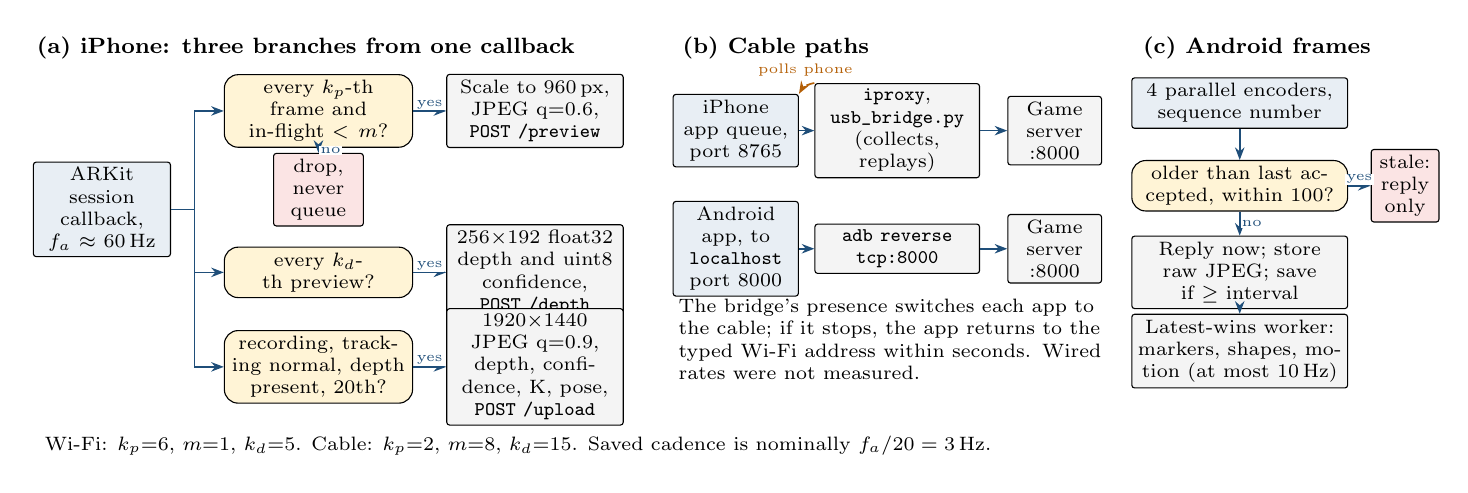
\begin{tikzpicture}[x=1cm,y=1cm]
\node[panel,anchor=west] at (-0.2,4.05) {(a) iPhone: three branches from one callback};
\node[hw,text width=1.6cm] (ar) at (0.75,2.0) {ARKit session callback, $f_a\approx60$\,Hz};
\node[dec,text width=2.25cm] (p1) at (3.5,3.25) {every $k_p$-th frame and in-flight $<m$?};
\node[box,text width=2.1cm] (p2) at (6.25,3.25) {Scale to 960\,px, JPEG q=0.6, \codes{POST /preview}};
\node[term,text width=1.0cm] (p3) at (3.5,2.25) {drop, never queue};
\node[dec,text width=2.25cm] (d1) at (3.5,1.2) {every $k_d$-th preview?};
\node[box,text width=2.1cm] (d2) at (6.25,1.2) {256$\times$192 float32 depth and uint8 confidence, \codes{POST /depth}};
\node[dec,text width=2.25cm] (s1) at (3.5,0.0) {recording, tracking normal, depth present, 20th?};
\node[box,text width=2.1cm] (s2) at (6.25,0.0) {1920$\times$1440 JPEG q=0.9, depth, confidence, K, pose, \codes{POST /upload}};
\draw[d] (ar.east) -- ++(0.3,0) |- (p1.west);
\draw[d] (ar.east) -- ++(0.3,0) |- (d1.west);
\draw[d] (ar.east) -- ++(0.3,0) |- (s1.west);
\draw[d] (p1) -- node[yes,above]{yes} (p2);
\draw[d] (p1) -- node[yes,right]{no} (p3);
\draw[d] (d1) -- node[yes,above]{yes} (d2);
\draw[d] (s1) -- node[yes,above]{yes} (s2);
\node[align=left,anchor=north west,font=\scriptsize] at (-0.1,-0.75) {Wi-Fi: $k_p{=}6$, $m{=}1$, $k_d{=}5$. Cable: $k_p{=}2$, $m{=}8$, $k_d{=}15$. Saved cadence is nominally $f_a/20=3$\,Hz.};
% panel b
\node[panel,anchor=west] at (8.0,4.05) {(b) Cable paths};
\node[hw,text width=1.45cm] (i1) at (8.8,3.0) {iPhone app queue, port 8765};
\node[box,text width=1.95cm] (i2) at (10.85,3.0) {\codes{iproxy}, \codes{usb_bridge.py} (collects, replays)};
\node[box,text width=1.05cm] (i3) at (12.85,3.0) {Game server :8000};
\draw[c] (i2.north west) to[bend right=25] node[above,font=\tiny]{polls phone} (i1.north east);
\draw[d] (i1) -- (i2); \draw[d] (i2) -- (i3);
\node[hw,text width=1.45cm] (a1) at (8.8,1.5) {Android app, to \codes{localhost} port 8000};
\node[box,text width=1.95cm] (a2) at (10.85,1.5) {\codes{adb reverse tcp:8000}};
\node[box,text width=1.05cm] (a3) at (12.85,1.5) {Game server :8000};
\draw[d] (a1) -- (a2); \draw[d] (a2) -- (a3);
\node[anchor=west,align=left,text width=5.5cm] at (7.95,0.35) {The bridge's presence switches each app to the cable; if it stops, the app returns to the typed Wi-Fi address within seconds. Wired rates were not measured.};
% panel c
\node[panel,anchor=west] at (13.85,4.05) {(c) Android frames};
\node[hw,text width=2.6cm] (c1) at (15.2,3.35) {4 parallel encoders, sequence number};
\node[dec,text width=2.6cm] (c2) at (15.2,2.3) {older than last accepted, within 100?};
\node[box,text width=2.6cm] (c3) at (15.2,1.2) {Reply now; store raw JPEG; save if $\geq$ interval};
\node[box,text width=2.6cm] (c4) at (15.2,0.2) {Latest-wins worker: markers, shapes, motion (at most 10\,Hz)};
\node[term,text width=0.72cm] (c5) at (17.3,2.3) {stale: reply only};
\draw[d] (c1) -- (c2); \draw[d] (c2) -- node[yes,right]{no} (c3); \draw[d] (c3) -- (c4);
\draw[d] (c2.east) -- node[yes,above]{yes} (c5.west);
\end{tikzpicture}
\caption{Acquisition. (a) iPhone decimation. (b) Wired relays for each phone. (c) Android stale-frame drop and the single-slot worker. Frames dropped here are never retried.}\label{fig:acq}
\end{figure*}

\subsection{Pose and overlay}\label{sec:pose}
Four 40\,mm \code{DICT_4X4_50} markers sit on a board around the tower. Fig.~\ref{fig:pose}(a) shows the frames: a point in the corrected tower frame reaches a camera through the optional LiDAR correction, $x_m=R_cx_\tau+t_c$, then the marker pose, $x_c=Rx_m+t$, and finally a per-camera edge delta. The correction applies only to the iPhone, because applying it to Android put that overlay a full layer too high \evO.

Fig.~\ref{fig:pose}(b) gives the solve. With four markers IPPE runs on marker centres; with three, SQPnP runs and 24 further seeded solves (8 azimuths, 3 elevations) produce candidates, because three centres admit several exact poses from a low camera. Candidates must place the camera above the board and fit centres within 2\,px, and the best is refined on corners with the per-marker rotation. Poses above 10\,px reprojection error are rejected. A phone on a stand is smoothed with an exponential average ($\alpha=0.2$), while a jump above 1.2$^\circ$ or 10\,mm is taken at once.

Fig.~\ref{fig:pose}(c) gives the tracking states. A good recent pose is reused when visible markers still land within 1.5\,px, with a full solve at least every 0.5\,s. When fewer than three markers are visible, the last pose holds for 1.5\,s, and the stored pose for up to 6\,s if the visible markers still agree. A \emph{lock} button freezes the overlay. Markers below 28\,px per side drop the pose and ask the user to move the phone.

\emph{Board calibration.} \code{tools/calibrate_board.py} solves every marker's 3-D corners and camera poses together, once, and writes \code{marker_map.json}. Without it the nominal layout is used.

\emph{Edge snapping.} After Re-detect, \code{tower_edges.refine} searches six small pose parameters on three frames, maximising the mean gradient across the projected box edges minus a penalty ($\sigma=8$\,mm, 2.5$^\circ$), coarse to fine. The median delta is kept only if at least two frames improve to $s_\mathrm{after}\geq1.15\,s_\mathrm{before}+0.5$.

\begin{figure*}[!t]\centering
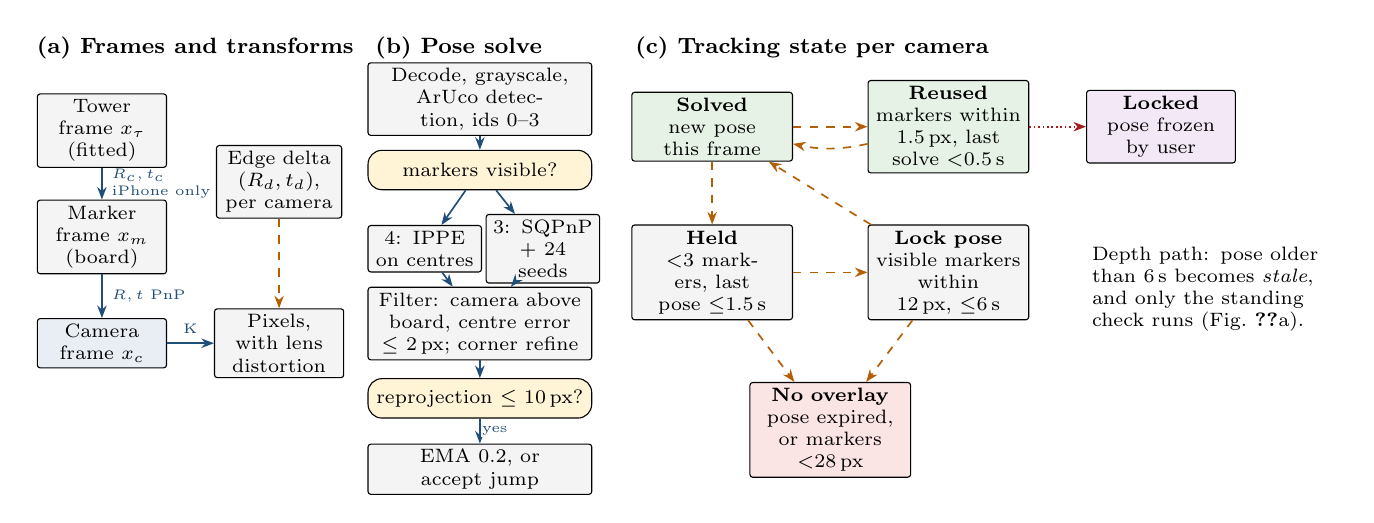
\begin{tikzpicture}[x=1cm,y=1cm]
\node[panel,anchor=west] at (-0.2,4.3) {(a) Frames and transforms};
\node[box,text width=1.5cm] (f1) at (0.75,3.25) {Tower frame $x_\tau$ (fitted)};
\node[box,text width=1.5cm] (f2) at (0.75,1.9) {Marker frame $x_m$ (board)};
\node[hw,text width=1.5cm] (f3) at (0.75,0.55) {Camera frame $x_c$};
\node[box,text width=1.5cm] (f4) at (3.0,0.55) {Pixels, with lens distortion};
\draw[d] (f1) -- node[right,font=\tiny,align=left]{$R_c,t_c$\\iPhone only} (f2);
\draw[d] (f2) -- node[right,font=\tiny]{$R,t$ PnP} (f3);
\draw[d] (f3) -- node[above,font=\tiny]{K} (f4);
\node[box,text width=1.45cm] (f5) at (3.0,2.6) {Edge delta $(R_d,t_d)$, per camera};
\draw[c] (f5) -- (f4);
% panel b
\node[panel,anchor=west] at (4.1,4.3) {(b) Pose solve};
\node[box,text width=2.7cm] (b1) at (5.55,3.65) {Decode, grayscale, ArUco detection, ids 0--3};
\node[dec,text width=2.7cm] (b2) at (5.55,2.75) {markers visible?};
\node[box,text width=1.3cm] (b3a) at (4.85,1.75) {4: IPPE on centres};
\node[box,text width=1.3cm] (b3b) at (6.35,1.75) {3: SQPnP + 24 seeds};
\node[box,text width=2.7cm] (b4) at (5.55,0.8) {Filter: camera above board, centre error $\leq2$\,px; corner refine};
\node[dec,text width=2.7cm] (b5) at (5.55,-0.15) {reprojection $\leq10$\,px?};
\node[box,text width=2.7cm] (b6) at (5.55,-1.05) {EMA 0.2, or accept jump};
\draw[d] (b1) -- (b2); \draw[d] (b2) -- (b3a); \draw[d] (b2) -- (b3b);
\draw[d] (b3a) -- (b4); \draw[d] (b3b) -- (b4); \draw[d] (b4) -- (b5); \draw[d] (b5) -- node[yes,right]{yes} (b6);
% panel c
\node[panel,anchor=west] at (7.4,4.3) {(c) Tracking state per camera};
\node[box,text width=1.9cm,fill=fstore] (s1) at (8.5,3.3) {\textbf{Solved}\\new pose this frame};
\node[box,text width=1.9cm,fill=fstore] (s2) at (11.5,3.3) {\textbf{Reused}\\markers within 1.5\,px, last solve $<$0.5\,s};
\node[box,text width=1.9cm] (s3) at (8.5,1.45) {\textbf{Held}\\$<$3 markers, last pose $\leq$1.5\,s};
\node[box,text width=1.9cm] (s4) at (11.5,1.45) {\textbf{Lock pose}\\visible markers within 12\,px, $\leq$6\,s};
\node[term,text width=1.9cm] (s5) at (10.0,-0.55) {\textbf{No overlay}\\pose expired, or markers $<$28\,px};
\node[box,text width=1.75cm,fill=fext] (s6) at (14.2,3.3) {\textbf{Locked}\\pose frozen by user};
\draw[c] (s1) -- (s2); \draw[c] (s2) to[bend left=12] (s1);
\draw[c] (s1) -- (s3); \draw[c] (s3) -- (s4); \draw[c] (s3) -- (s5); \draw[c] (s4) -- (s5);
\draw[c] (s4) -- (s1);
\draw[h] (s2) -- (s6);
\node[anchor=north west,text width=3.1cm,align=left] at (13.2,1.9) {Depth path: pose older than 6\,s becomes \emph{stale}, and only the standing check runs (Fig.~\ref{fig:depth}a).};
\end{tikzpicture}
\caption{Pose. (a) Transform chain; the LiDAR correction is applied only on the iPhone. (b) Solve with its rejection filters. (c) Simplified per-camera states, from \protect\code{_draw_overlay}.}\label{fig:pose}
\end{figure*}

\subsection{Depth path}\label{sec:depth}
Each depth frame (Fig.~\ref{fig:depth}a) is ignored while a hand is active. Otherwise, high-confidence pixels (confidence $\geq2$, $0.05<d<1.5$\,m) are back-projected, $X=(u-c_x)d/f_x$, $Y=(v-c_y)d/f_y$, $Z=d$, and mapped into the tower frame, $P=R^\top(X-t)$.

\emph{Tower fit.} \code{tower_fit.fit_box} fits $\theta=(t,r,H)$: shift, rotation vector and height of a 75$\times$75\,mm box, with an annular ring of board points. Residuals are the box signed distance and the ring's height. For each $\sigma\in\{30,20,12,8,5\}$\,mm it runs six damped Gauss--Newton steps with a numerical Jacobian and weights $w_i=(\sigma^2/(\sigma^2+r_i^2))^2$ (Algorithm~1). A result is accepted if inliers ($|r|<4$\,mm) reach 55\,\%, RMS is at most 4\,mm, and $H$ stays within 12\,mm of the running median. Only 60\,\% of each accepted step is applied. After convergence only tiny corrections are believed, and 20 steady disagreements reset the fit. Layer count is $\mathrm{round}(H/15\,\mathrm{mm})$.

\emph{Loose blocks.} A face's first six readings form its baseline, unless they scatter by more than 3\,mm. A median protrusion of at least 5\,mm (and at most 30\,mm) on two consecutive checks turns an allowed block amber. This has been tested only on injected offsets, not a real loose block \evU.

\begin{figure}[!t]\centering\footnotesize
\begin{minipage}{\columnwidth}\hrule\smallskip
\textbf{Algorithm 1:} \texttt{fit\_box}$(P)$\smallskip\hrule\smallskip
\begin{tabbing}
\hspace{3mm}\=\hspace{3mm}\=\hspace{3mm}\=\kill
split $P$ into near points (tower window) and ring points\\
\textbf{if} fewer than 300 near points \textbf{return} none\\
cap to 2500 near and 1250 ring points\\
$\theta\gets0$;\ $H\gets$ 98th percentile of near-point height\\
\textbf{for} $\sigma$ in 30, 20, 12, 8, 5 mm \textbf{do}\\
\>\textbf{repeat} 6 times\\
\>\>$r\gets$ residuals$(\theta)$;\ $w\gets(\sigma^2/(\sigma^2+r^2))^2$\\
\>\>$J\gets$ numerical Jacobian of $r$\\
\>\>$\delta\gets-(J^\top WJ+10^{-3}I)^{-1}J^\top Wr$\\
\>\>$\theta\gets\theta+\mathrm{clip}(\delta)$\\
\textbf{return} $R(\theta),t,H$, inlier share, RMS
\end{tabbing}\hrule
\end{minipage}
\end{figure}

\begin{figure*}[!t]\centering
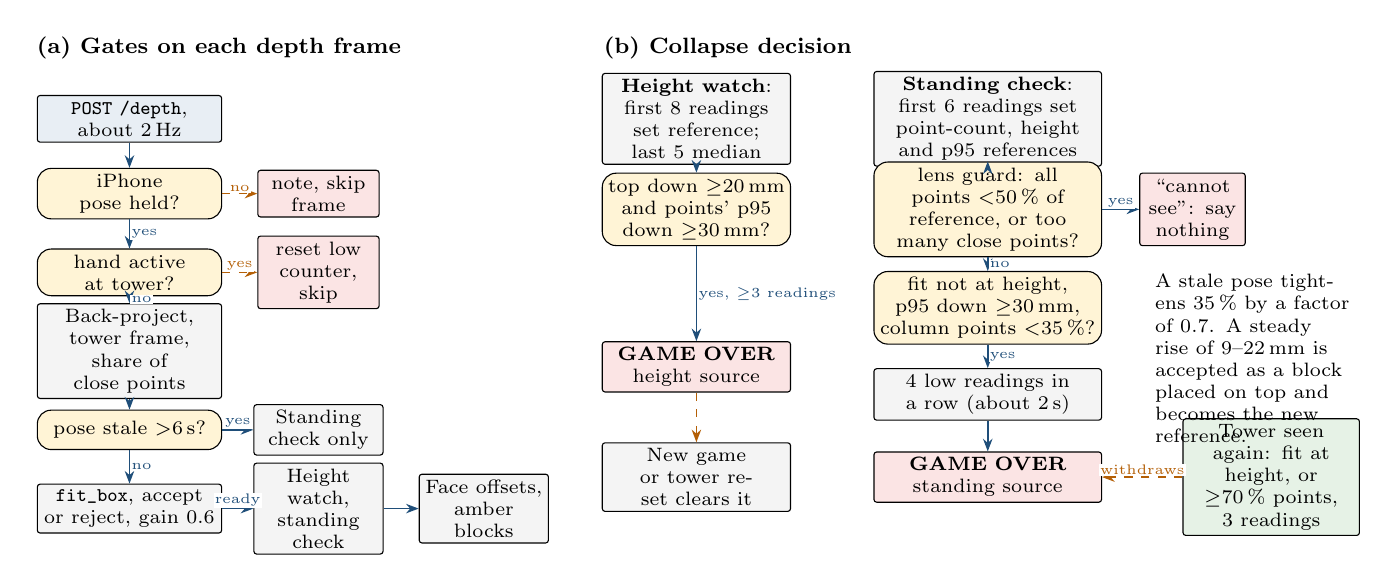
\begin{tikzpicture}[x=1cm,y=1cm]
\node[panel,anchor=west] at (-0.2,5.25) {(a) Gates on each depth frame};
\node[hw,text width=2.2cm] (a0) at (1.1,4.35) {\codes{POST /depth}, about 2\,Hz};
\node[dec,text width=2.2cm] (a1) at (1.1,3.4) {iPhone pose held?};
\node[dec,text width=2.2cm] (a2) at (1.1,2.4) {hand active at tower?};
\node[box,text width=2.2cm] (a3) at (1.1,1.4) {Back-project, tower frame, share of close points};
\node[dec,text width=2.2cm] (a4) at (1.1,0.4) {pose stale $>$6\,s?};
\node[box,text width=2.2cm] (a5) at (1.1,-0.6) {\codes{fit_box}, accept or reject, gain 0.6};
\node[term,text width=1.4cm] (t1) at (3.5,3.4) {note, skip frame};
\node[term,text width=1.4cm] (t2) at (3.5,2.4) {reset low counter, skip};
\node[box,text width=1.5cm] (t3) at (3.5,0.4) {Standing check only};
\node[box,text width=1.5cm] (a6) at (3.5,-0.6) {Height watch, standing check};
\node[box,text width=1.5cm] (a7) at (5.6,-0.6) {Face offsets, amber blocks};
\draw[d] (a0) -- (a1); \draw[d] (a1) -- node[yes,right]{yes} (a2); \draw[d] (a2) -- node[yes,right]{no} (a3);
\draw[d] (a3) -- (a4); \draw[d] (a4) -- node[yes,right]{no} (a5);
\draw[c] (a1) -- node[yes,above]{no} (t1); \draw[c] (a2) -- node[yes,above]{yes} (t2);
\draw[d] (a4) -- node[yes,above]{yes} (t3);
\draw[d] (a5) -- node[yes,above]{ready} (a6); \draw[d] (a6) -- (a7);
% panel b
\node[panel,anchor=west] at (7.0,5.25) {(b) Collapse decision};
\node[box,text width=2.25cm] (h1) at (8.3,4.35) {\textbf{Height watch}: first 8 readings set reference; last 5 median};
\node[dec,text width=2.25cm] (h2) at (8.3,3.2) {top down $\geq$20\,mm and points' p95 down $\geq$30\,mm?};
\node[box,text width=2.75cm] (s1) at (12.0,4.35) {\textbf{Standing check}: first 6 readings set point-count, height and p95 references};
\node[dec,text width=2.75cm] (s2) at (12.0,3.2) {lens guard: all points $<$50\,\% of reference, or too many close points?};
\node[term,text width=1.2cm] (s3) at (14.6,3.2) {``cannot see'': say nothing};
\node[dec,text width=2.75cm] (s4) at (12.0,1.95) {fit not at height, p95 down $\geq$30\,mm, column points $<$35\,\%?};
\node[box,text width=2.75cm] (s5) at (12.0,0.85) {4 low readings in a row (about 2\,s)};
\node[term,text width=2.25cm] (g1) at (8.3,1.2) {\textbf{GAME OVER}\\height source};
\node[term,text width=2.75cm] (g2) at (12.0,-0.2) {\textbf{GAME OVER}\\standing source};
\node[box,text width=2.1cm,fill=fstore] (g3) at (15.6,-0.2) {Tower seen again: fit at height, or $\geq$70\,\% points, 3 readings};
\node[box,text width=2.25cm] (g4) at (8.3,-0.2) {New game or tower reset clears it};
\draw[d] (h1) -- (h2); \draw[d] (h2) -- node[yes,right]{yes, $\geq$3 readings} (g1); \draw[c] (g1) -- (g4);
\draw[d] (s1) -- (s2); \draw[d] (s2) -- node[yes,above]{yes} (s3); \draw[d] (s2) -- node[yes,right]{no} (s4);
\draw[d] (s4) -- node[yes,right]{yes} (s5); \draw[d] (s5) -- (g2);
\draw[c] (g3) -- node[yes,above]{withdraws} (g2);
\node[anchor=north west,text width=2.5cm,align=left] at (14.0,2.5) {A stale pose tightens 35\,\% by a factor of 0.7. A steady rise of 9--22\,mm is accepted as a block placed on top and becomes the new reference.};
\end{tikzpicture}
\caption{Depth. (a) Frame gating. (b) The two collapse paths. Only the standing-check alarm clears itself; the height-watch alarm stays until the tower is reset.}\label{fig:depth}
\end{figure*}

\subsection{Hand presence and comparison windows}\label{sec:hand}
The game server does not run a hand model. Hand presence is inferred from frame differencing over the tower: each analysed frame is reduced to 192$\times$108 grayscale, and if the share of pixels in the tower region (the projected box enlarged by 40\,\%) changing by more than 22 grey levels exceeds \code{MOTION_FRAC} (0.06 iPhone, 0.10 Android), an activity event is recorded. Activity holds for 0.8\,s and stops counting after 15\,s of continuous motion, so flicker cannot wait forever. This is not a person detector: any large change in the region counts.

Events closer than 3\,s form one burst (Fig.~\ref{fig:finder}a). For a MARK, the move is the last burst that began before the tap. The ``after'' window is the first calm stretch after it, starting 0.4\,s after the burst and lasting up to 1.6\,s, ending early if the next burst (a block being placed) begins. The ``before'' window is up to 3.2\,s, ending 0.3\,s before the burst. On a quiet game the older clock windows (1.0--4.5\,s after the previous tap and 0.8--2.5\,s after this tap) are kept when no block has been placed since and neither contains activity.

\subsection{Pull identification with \texttt{move\_infer}}\label{sec:finder}
Fig.~\ref{fig:finder}(b) and Algorithm~2 show the deployed finder. While data capture is on, 100$\times$60 crops of block end and side faces are cut for each frame, skipping near edge-on views. For camera $c$, face $f$ and window $W$, up to 12 crops are blurred, normalised to zero mean and unit variance, and averaged into $\bar I^W_{cf}$, needing at least two crops. A face must appear in both windows.

The after image is registered to the before image by phase correlation with a Hann window, with the shift clipped so that a small tower movement does not count. The residual is the mean absolute difference in the face core,
\begin{equation}
e_{cf}=\frac{1}{|\Omega|}\sum_{p\in\Omega}\bigl|\bar I^{a}_{cf}(p)-\bar I^{b}_{cf}(p+\hat d)\bigr|.
\end{equation}
Each crop kind $\kappa$ (end or side) has its own robust baseline, pooled over the cameras seen,
\begin{equation}
z_{cf}=\frac{e_{cf}-\mathrm{med}_\kappa(e)}{1.4826\,\mathrm{MAD}_\kappa(e)+10^{-3}}.
\end{equation}
A block's score in a camera is the largest $z$ among its faces, and the block score is the \emph{unweighted} camera mean,
\begin{equation}
S_{\ell s}=\begin{cases}\tfrac12\bigl(\max_{f}z_{\mathrm{i},f}+\max_{f}z_{\mathrm{a},f}\bigr) & \text{both cameras,}\\ \max_{f}z_{c,f}-2 & \text{one camera.}\end{cases}
\end{equation}
The reasoning in the code is that a hole is seen by both cameras, whereas a hand or shadow usually fools one.

\emph{Free mode} (after each MARK) ranks legal candidates: standing blocks below the top complete layer. With best score $z_1$ and gap $g$ to the best block of any other layer, the confidence is a lookup: (12, 6)$\to$95\,\%, (10, 5)$\to$91\,\%, (8, 4)$\to$88\,\%, (6, 3)$\to$84\,\%, otherwise 50\,\%. At 90\,\% or more the block enters the ledger at once and the player answers Yes or No. No undoes it. Below 90\,\% nothing changes and the player types the move (Fig.~\ref{fig:finder}c).

\emph{Typed mode} restricts scoring to the typed column and may swap left and right if the other outer column clearly stands out. Its tiers are (10, 5)$\to$92\,\%, (8, 4)$\to$89\,\%, (5, 3)$\to$85\,\%, (3, 2)$\to$82\,\%, otherwise 44\,\%. Its answer is applied if $z\geq3$, $g\geq2$ and the tier is at least 75\,\%, so a typed-path answer can be applied below the free path's 90\,\% gate. A typed layer always counts.

These percentages are in-sample lookups. Source comments say they were tabulated from 57 moves in 12 games using the same optimistic labels, so they are not calibrated probabilities in the sense of~\cite{guo2017}, and the paper does not use them as evidence of accuracy.

\begin{figure*}[!t]\centering
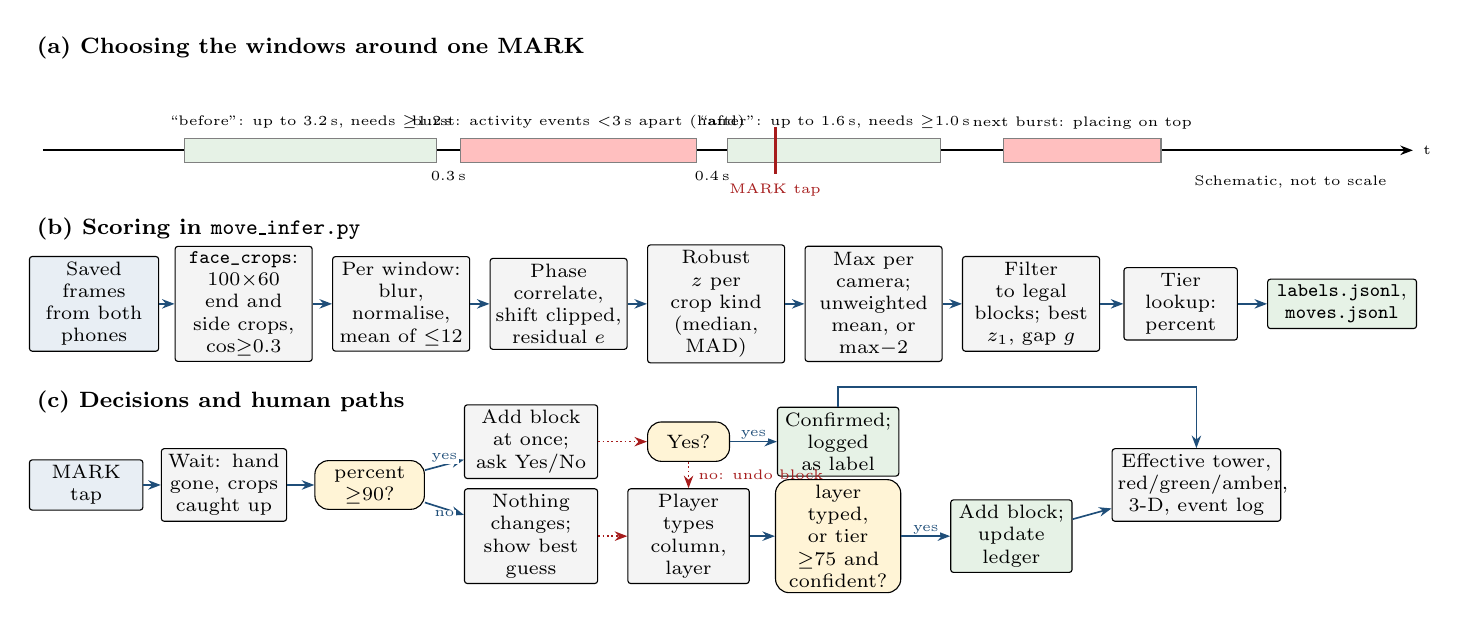
\begin{tikzpicture}[x=1cm,y=1cm]
\node[panel,anchor=west] at (-0.2,6.0) {(a) Choosing the windows around one MARK};
\draw[->,thick] (0,4.7) -- (17.4,4.7) node[right,font=\tiny]{t};
\fill[fstore,draw=gray] (1.8,4.55) rectangle (5.0,4.85);
\node[above,font=\tiny,align=center] at (3.4,4.85) {``before'': up to 3.2\,s, needs $\geq$1.2\,s};
\fill[red!25,draw=gray] (5.3,4.55) rectangle (8.3,4.85);
\node[above,font=\tiny,align=center] at (6.8,4.85) {burst: activity events $<$3\,s apart (hand)};
\fill[fstore,draw=gray] (8.7,4.55) rectangle (11.4,4.85);
\node[above,font=\tiny,align=center] at (10.05,4.85) {``after'': up to 1.6\,s, needs $\geq$1.0\,s};
\fill[red!25,draw=gray] (12.2,4.55) rectangle (14.2,4.85);
\node[above,font=\tiny] at (13.2,4.85) {next burst: placing on top};
\draw[chum,very thick] (9.3,4.4) -- (9.3,5.0);
\node[below,font=\tiny,chum] at (9.3,4.4) {MARK tap};
\node[below,font=\tiny] at (5.15,4.55) {0.3\,s};
\node[below,font=\tiny] at (8.5,4.55) {0.4\,s};
\node[font=\tiny,anchor=west] at (14.5,4.3) {Schematic, not to scale};
% panel b
\node[panel,anchor=west] at (-0.2,3.7) {(b) Scoring in \texttt{move\_infer.py}};
\node[hw,text width=1.5cm] (b0) at (0.65,2.75) {Saved frames from both phones};
\node[box,text width=1.6cm] (b1) at (2.55,2.75) {\codes{face_crops}: 100$\times$60 end and side crops, cos$\geq$0.3};
\node[box,text width=1.6cm] (b2) at (4.55,2.75) {Per window: blur, normalise, mean of $\leq$12};
\node[box,text width=1.6cm] (b3) at (6.55,2.75) {Phase correlate, shift clipped, residual $e$};
\node[box,text width=1.6cm] (b4) at (8.55,2.75) {Robust $z$ per crop kind (median, MAD)};
\node[box,text width=1.6cm] (b5) at (10.55,2.75) {Max per camera; unweighted mean, or max$-$2};
\node[box,text width=1.6cm] (b6) at (12.55,2.75) {Filter to legal blocks; best $z_1$, gap $g$};
\node[box,text width=1.3cm] (b7) at (14.45,2.75) {Tier lookup: percent};
\draw[d] (b0)--(b1); \draw[d] (b1)--(b2); \draw[d] (b2)--(b3); \draw[d] (b3)--(b4); \draw[d] (b4)--(b5); \draw[d] (b5)--(b6); \draw[d] (b6)--(b7);
\node[store,text width=1.75cm] (b8) at (16.5,2.75) {\codes{labels.jsonl}, \codes{moves.jsonl}};
\draw[d] (b7)--(b8);
% panel c
\node[panel,anchor=west] at (-0.2,1.5) {(c) Decisions and human paths};
\node[hw,text width=1.3cm] (c0) at (0.55,0.45) {MARK tap};
\node[box,text width=1.45cm] (c1) at (2.3,0.45) {Wait: hand gone, crops caught up};
\node[dec,text width=1.25cm] (c2) at (4.15,0.45) {percent $\geq$90?};
\node[box,text width=1.55cm] (c3) at (6.2,1.0) {Add block at once; ask Yes/No};
\node[box,text width=1.55cm] (c4) at (6.2,-0.2) {Nothing changes; show best guess};
\node[dec,text width=0.9cm] (c5) at (8.2,1.0) {Yes?};
\node[store,text width=1.4cm] (c6) at (10.1,1.0) {Confirmed; logged as label};
\node[box,text width=1.4cm] (c7) at (8.2,-0.2) {Player types column, layer};
\node[dec,text width=1.45cm] (c8) at (10.1,-0.2) {layer typed, or tier $\geq$75 and confident?};
\node[store,text width=1.4cm] (c9) at (12.3,-0.2) {Add block; update ledger};
\node[box,text width=2.0cm] (c10) at (14.65,0.45) {Effective tower, red/green/amber, 3-D, event log};
\draw[d] (c0)--(c1); \draw[d] (c1)--(c2);
\draw[d] (c2) -- node[yes,above]{yes} (c3); \draw[d] (c2) -- node[yes,below]{no} (c4);
\draw[h] (c3)--(c5); \draw[d] (c5)--node[yes,above]{yes}(c6);
\draw[h] (c5.south) -- node[right,font=\tiny]{no: undo block} (c7.north);
\draw[h] (c4)--(c7); \draw[d] (c7)--(c8); \draw[d] (c8)--node[yes,above]{yes}(c9); \draw[d] (c9)--(c10);
\draw[d] (c6.north) -- ++(0,0.25) -| (c10.north);
\end{tikzpicture}
\caption{Pull identification. (a) Window selection from frame-difference activity. (b) Scoring in the deployed finder. (c) The Yes/No path (at least 90\,\%) and the typed path. A ``No'' undoes the block and returns to typing.}\label{fig:finder}
\end{figure*}

\begin{figure}[!t]\centering\footnotesize
\begin{minipage}{\columnwidth}\hrule\smallskip
\textbf{Algorithm 2:} \texttt{infer\_free} and its gate\smallskip\hrule\smallskip
\begin{tabbing}
\hspace{3mm}\=\hspace{3mm}\=\kill
$S\gets$ block scores for faces in both windows\\
\textbf{if} fewer than 10 common faces \textbf{return} ask player\\
keep blocks that could legally have been pulled\\
\textbf{if} fewer than 3 remain \textbf{return} ask player\\
$(\ell^\ast,s^\ast)\gets\arg\max S$;\ $z_1\gets S_{\ell^\ast s^\ast}$\\
$z_2\gets$ best score in any other layer;\ $g\gets z_1-z_2$\\
$p\gets$ tier$(z_1,g)$\\
\textbf{if} $p\geq90$ \textbf{then} add block, ask Yes/No\\
\textbf{else} keep tower, ask player to type
\end{tabbing}\hrule
\end{minipage}
\end{figure}

\subsection{Balance rule and legality}\label{sec:balance}
Blocks are coloured by \code{jenga_rules.py}. Only layers below the highest complete layer may be pulled, and the bottom layer is excluded by a house rule. After a hypothetical pull, for every layer $j$ the centre of mass $\bar c_j$ of all blocks above must lie inside that layer's footprint $F_j$ with margin $\mu=4$\,mm:
\begin{equation}
\bar c_j\in F_j\ominus\mu,\quad \text{for all } j \text{ with blocks above},
\end{equation}
where $F_j$ spans from the outer edge of the lowest remaining slot to the outer edge of the highest, over the full 75\,mm length. A layer may never be emptied. The model assumes equal block weight and no friction. A tower already out of balance above a layer freezes everything below it, which is what produces ``no moves left''. Algorithm~3 states the check and Fig.~\ref{fig:balance} works through one layer.

\begin{figure}[!t]\centering\footnotesize
\begin{minipage}{\columnwidth}\hrule\smallskip
\textbf{Algorithm 3:} may block $(\ell,s)$ be pulled?\smallskip\hrule\smallskip
\begin{tabbing}
\hspace{3mm}\=\hspace{3mm}\=\kill
\textbf{if} $\ell=0$ \textbf{return} no (house rule)\\
\textbf{if} $\ell\geq$ top complete layer \textbf{return} no\\
remove $(\ell,s)$ from the standing set\\
\textbf{for} each layer $j$ with blocks above \textbf{do}\\
\>\textbf{if} layer $j$ is empty \textbf{return} no\\
\>$\bar c_j\gets$ mean of block centres above $j$\\
\>\textbf{if} $\bar c_j\notin F_j\ominus 4$\,mm \textbf{return} no\\
\textbf{return} yes
\end{tabbing}\hrule
\end{minipage}
\end{figure}

\begin{figure}[!t]\centering
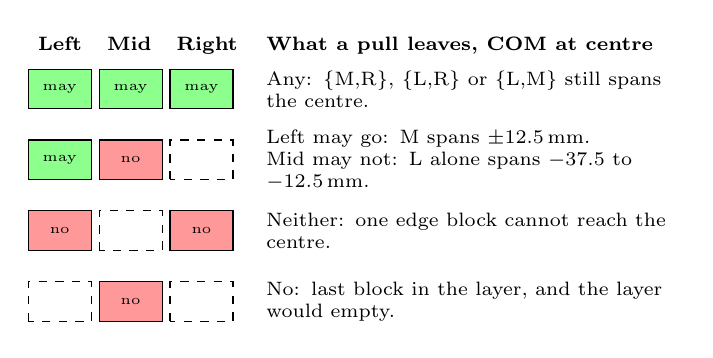
\begin{tikzpicture}[x=1mm,y=1mm]
\newcommand{\slotrow}[5]{%
 \node[anchor=east,font=\scriptsize] at (#1-2,#2+2.5) {#3};
 \foreach \s/\v in {0/#4} {\ifnum\v=1\fill[green!45!white,draw=black] (#1+0,#2) rectangle ++(9,5);\else\ifnum\v=2\fill[red!40!white,draw=black] (#1+0,#2) rectangle ++(9,5);\else\draw[black,dashed] (#1+0,#2) rectangle ++(9,5);\fi\fi}
 \node[anchor=west,font=\scriptsize,text width=44mm,align=left] at (#1+30,#2+2.5) {#5};}
\newcommand{\cell}[3]{\ifnum#3=1\fill[green!45!white,draw=black] (#1,#2) rectangle ++(8,5);\node[font=\tiny] at (#1+4,#2+2.5){may};\else\ifnum#3=2\fill[red!40!white,draw=black] (#1,#2) rectangle ++(8,5);\node[font=\tiny] at (#1+4,#2+2.5){no};\else\draw[black,dashed] (#1,#2) rectangle ++(8,5);\fi\fi}
\node[font=\scriptsize\bfseries,anchor=west] at (0,41) {Left\quad Mid\quad Right};
\node[font=\scriptsize\bfseries,anchor=west] at (29,41) {What a pull leaves, COM at centre};
\cell{0}{33}{1}\cell{9}{33}{1}\cell{18}{33}{1}
\node[anchor=west,text width=52mm,align=left] at (29,35.5) {Any: \{M,R\}, \{L,R\} or \{L,M\} still spans the centre.};
\cell{0}{24}{1}\cell{9}{24}{2}\cell{18}{24}{0}
\node[anchor=west,text width=52mm,align=left] at (29,26.5) {Left may go: M spans $\pm$12.5\,mm. Mid may not: L alone spans $-37.5$ to $-12.5$\,mm.};
\cell{0}{15}{2}\cell{9}{15}{0}\cell{18}{15}{2}
\node[anchor=west,text width=52mm,align=left] at (29,17.5) {Neither: one edge block cannot reach the centre.};
\cell{0}{6}{0}\cell{9}{6}{2}\cell{18}{6}{0}
\node[anchor=west,text width=52mm,align=left] at (29,8.5) {No: last block in the layer, and the layer would empty.};
\end{tikzpicture}
\caption{Worked balance cases for one layer of a straight tower (dashed: gone). Slot centres are at $-25$, $0$ and $+25$\,mm. Checked by \protect\code{tests/test_jenga_rules.py}.}\label{fig:balance}
\end{figure}

\subsection{One move, end to end}
Fig.~\ref{fig:seq} follows one move. Only configured waits are shown. The player-visible time from MARK to answer was not logged in live games, so no end-to-end latency is claimed.

\begin{figure*}[!t]\centering
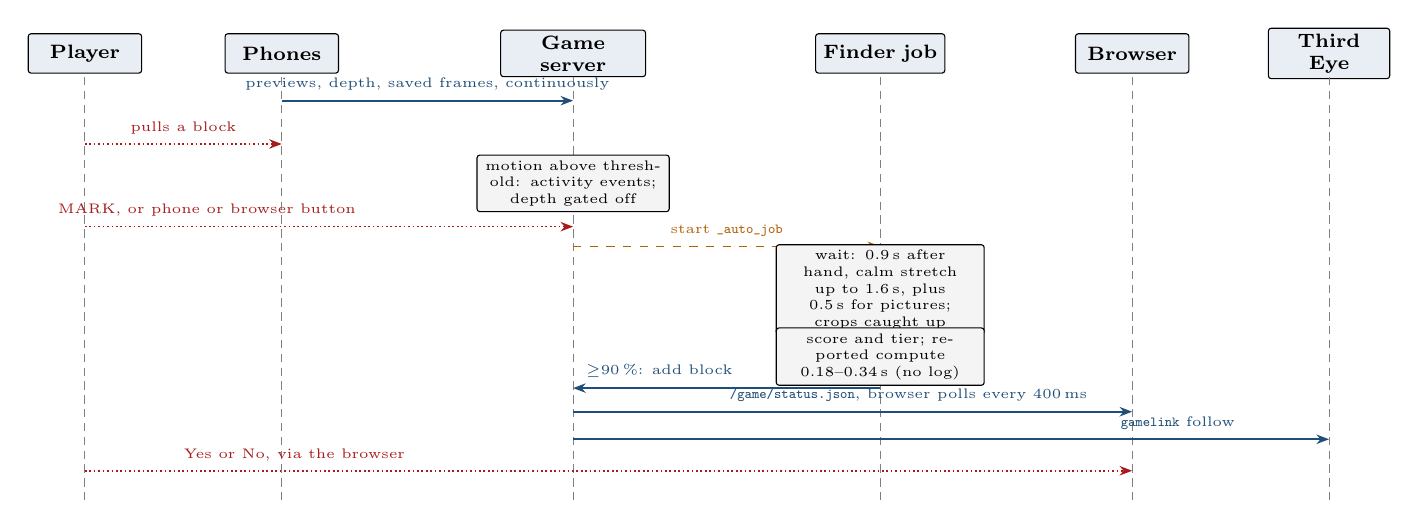
\begin{tikzpicture}[x=1cm,y=1cm]
\foreach \x/\n/\w in {0.9/Player/1.3,3.4/Phones/1.3,7.1/{Game server}/1.7,11.0/{Finder job}/1.5,14.2/Browser/1.3,16.7/{Third Eye}/1.4}{
 \node[hw,text width=\w cm] at (\x,5.2) {\textbf{\n}};
 \draw[gray,densely dashed] (\x,4.9) -- (\x,-0.5);}
\draw[d] (3.4,4.6) -- node[above,font=\tiny]{previews, depth, saved frames, continuously} (7.1,4.6);
\draw[h] (0.9,4.05) -- node[above,font=\tiny]{pulls a block} (3.4,4.05);
\node[box,text width=2.3cm,font=\tiny] at (7.1,3.55) {motion above threshold: activity events; depth gated off};
\draw[h] (0.9,3.0) -- node[above,font=\tiny,pos=0.25]{MARK, or phone or browser button} (7.1,3.0);
\draw[c] (7.1,2.75) -- node[above,font=\tiny]{start \codes{_auto_job}} (11.0,2.75);
\node[box,text width=2.5cm,font=\tiny] at (11.0,2.2) {wait: 0.9\,s after hand, calm stretch up to 1.6\,s, plus 0.5\,s for pictures; crops caught up};
\node[box,text width=2.5cm,font=\tiny] at (11.0,1.35) {score and tier; reported compute 0.18--0.34\,s (no log)};
\draw[d] (11.0,0.95) -- node[above,font=\tiny,pos=0.72]{$\geq$90\,\%: add block} (7.1,0.95);
\draw[d] (7.1,0.65) -- node[above,font=\tiny,pos=0.6]{\codes{/game/status.json}, browser polls every 400\,ms} (14.2,0.65);
\draw[d] (7.1,0.3) -- node[above,font=\tiny,pos=0.8]{\codes{gamelink} follow} (16.7,0.3);
\draw[h] (0.9,-0.1) -- node[above,font=\tiny,pos=0.2]{Yes or No, via the browser} (14.2,-0.1);
\end{tikzpicture}
\caption{Chronology of one move on the automatic path. Dotted: human. Waits are configured values from the source, not measured latencies; the compute range is a reported figure without an original log.}\label{fig:seq}
\end{figure*}

\subsection{Interface and computational cost}
The web app has a Game page, a 3-D tower page and a Replay page (Fig.~\ref{fig:ui}); the replay rebuilds a game from \code{moves.jsonl}. Back-projection is $\Theta(N)$. Each Gauss--Newton step evaluates residuals eight times over a capped point set, so the fit is bounded regardless of depth size. Face offsets cost $\Theta(LN)$. The referee considers up to $3L$ pulls, each checking $L$ layers with up to $3L$ blocks above, so it is $\Theta(L^3)$. A reported log-log slope of 2.80 is consistent with this. Exceptions in depth handling are caught and the reply is still \code{OK}, so a failed depth frame is lost silently.

\begin{figure}[!t]\centering
\includegraphics[height=3.25cm]{fig_overlay.png}\hspace{8mm}
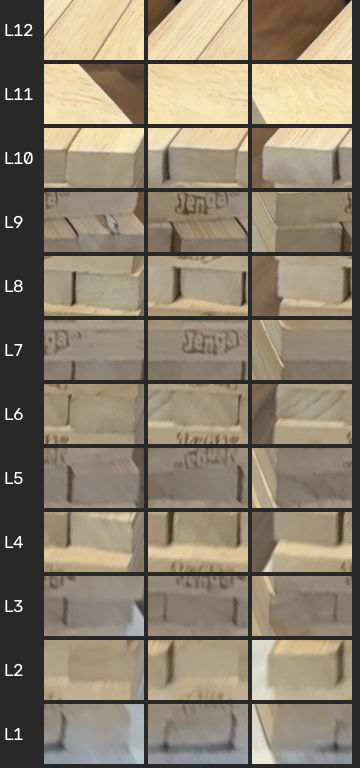
\includegraphics[height=3.25cm]{crops_montage_iphone.png}\\[3pt]
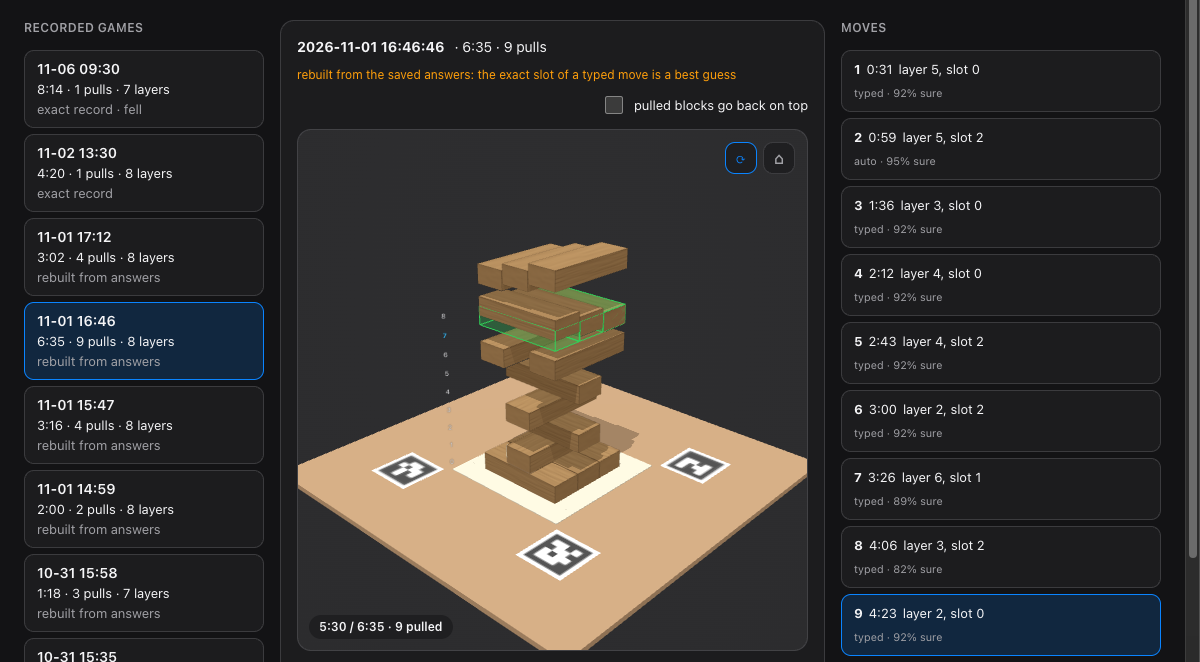
\includegraphics[width=\columnwidth]{fig_replay.png}
\caption{Top left: overlay on the iPhone view. Top right: end-face crops by layer from one recorded game. Bottom: Replay page for a recorded 8-layer game; ``typed'' and ``auto'' show which path resolved each move.}\label{fig:ui}
\end{figure}

\begin{table}[!t]
\caption{Key constants as deployed, with locations.}\label{tab:constants}
\centering\footnotesize
\begin{tabular}{@{}p{3.75cm}p{1.75cm}p{2.2cm}@{}}
\toprule
Quantity & Value & Location \\
\midrule
Save / preview / depth decimation & 20 / 6 or 2 / 5 or 15 & \codes{ViewController} \\
Overlay analysis cap & 10\,Hz per phone & \codes{ANALYSIS_FPS} \\
Pose EMA $\alpha$ & 0.2 & \codes{POSE_EMA} \\
Reuse threshold, full-solve period & 1.5\,px, 0.5\,s & \codes{REUSE_PX, REUSE_S} \\
Fit gates: inliers, RMS, height & 55\,\%, 4\,mm, 12\,mm & \codes{_fit_tower} \\
Motion threshold (iPhone, Android) & 0.06, 0.10 & \codes{MOTION_FRAC} \\
Activity hold, cap & 0.8\,s, 15\,s & \codes{ACTIVITY_*} \\
Finder clock window after tap & 0.8--2.5\,s & \codes{AFTER_S} \\
Automatic apply (free path) & $\geq$90\,\% & \codes{AUTO_PCT} \\
Typed-path apply & $\geq$75\,\% & \codes{AUTO_APPLY_PCT} \\
Balance margin & 4\,mm & \codes{MARGIN} \\
Collapse: top drop, p95 drop & 20\,mm, 30\,mm & \codes{DROP_MM, PTOP_DROP_MM} \\
Standing: points, readings & 35\,\%, 4 & \codes{STAND_*} \\
Loose threshold & 5\,mm & \codes{LOOSE_MM} \\
\bottomrule
\end{tabular}
\end{table}

\section{Evaluation Methodology}\label{sec:method}
This is an engineering case study in the sense of~\cite{runeson2009}: one system, one setup, examined with several kinds of evidence. Nothing is trained, so there is no train/test split, and no user study was run. The participants were the authors, and all constants were chosen on the same sessions evaluated here.

\subsection{Classes of evidence}
Each result has an \emph{evidence class} and a \emph{provenance}. Classes: \evM\ (from recorded experimental data), \evO\ (documented behaviour without sufficient quantitative evaluation), \evE\ (preliminary or post-hoc), \evU\ (contradictory or insufficient), and \evP\ (future work).

Provenance distinguishes four kinds, and we never call one by another's name:
\begin{itemize}
\item \textbf{Stored output}: machine-written files in a repository, namely \code{variant_scores.json} and upstream \code{eval/results/}.
\item \textbf{Transcribed}: \code{benchmarks/logs/*.txt}, copied from terminal output after the original files were lost. They are not original raw logs.
\item \textbf{Re-derived}: recalculated by us from stored output, or re-run by the team. We recomputed all finder tallies from the stored scores.
\item \textbf{Reported}: stated in the analysis files or the earlier paper draft, with no log available.
\end{itemize}

\subsection{Data}
Recordings exist only on one team member's computer (about 7.4\,GB) and are not public because they show identifiable people and rooms. We did not access them; all new calculations here use stored scores. Table~\ref{tab:experiments} lists every experiment, and Fig.~\ref{fig:evidence} shows how they feed each research question. Results under different detectors or conditions are never pooled.

\begin{table*}[!t]
\caption{Experiment register. Results in different rows are not interchangeable.}\label{tab:experiments}
\centering\footnotesize
\begin{tabular}{@{}p{0.45cm}p{3.75cm}p{5.0cm}p{2.3cm}p{2.0cm}p{2.5cm}@{}}
\toprule
ID & Experiment & Conditions & Sample & Class & Provenance \\
\midrule
E1 & Saved-frame acquisition & Three iPhone games & 1{,}706 frames & \evM & Reported, no log \\
E2 & Per-stage latency & Laptop CPU, one thread; another machine & 80 frames & \evM & Reported, no log \\
E3 & Finder, complete offline set & \code{eval_variants.py}, 3.0\,s after-window & 32 pulls, 11 games & \evM & Stored output, re-derived \\
E4 & Finder, historical snapshot & Same code when the draft was written & 31 pulls, 10 games & \evM & Re-derived subset of E3 \\
E5 & Finder, earlier label set & Older labels; cause of difference unrecorded & 57 pulls, 12 games & \evU & Reported, percentages only \\
E6 & Current server replay & Auto job on recorded frames, Mac & 5 and 10 moves & \evM & Reported, no log \\
E7 & Tall-tower replay & Old 16-layer games, before board calibration, current finder & 7 known moves & \evM & Reported, no log \\
E8 & Tall-tower historical & One fresh game, 25 Oct, finder of that date & 9 moves & \evO & Reported, README \\
E9 & Pose comparison & \code{benchmark_pose.py}, 3 towers, hand-free & 75 frames & \evM & Transcribed \\
E10 & Height comparison & \code{benchmark_height.py}, plus synthetic stress & 233 frames, 15 trials per level & \evM & Transcribed \\
E11 & Edge snapping, Android & Four sessions, enough markers & 5 frames & \evE & Reported, no log \\
E12 & Collapse, current detector & Three depth replays through server functions & 1 real fall, 3 games & \evM & Reported, no log \\
E13 & Collapse, older detector & Height-only detector, 25 Oct & 3 falls, 1 clean game & \evO & Reported, README \\
E14 & Depth-only pull finding & One camera, upstream evaluation & 10 pulls & \evM & Upstream document \\
E15 & Rule compiler (upstream) & 16-entry corpus; model-dependent & 16 entries, 80 claims & \evM & Stored upstream output \\
\bottomrule
\end{tabular}
\end{table*}

\begin{figure*}[!t]\centering
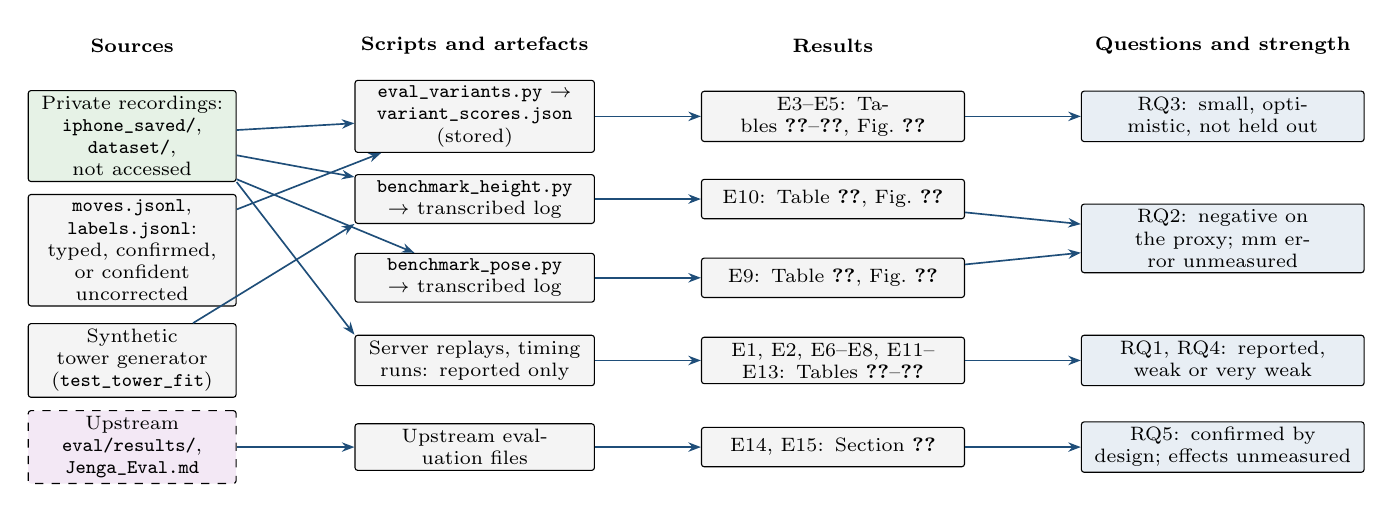
\begin{tikzpicture}[x=1cm,y=1cm]
\foreach \x/\t in {1.35/Sources,5.7/Scripts and artefacts,10.25/Results,15.2/Questions and strength}{\node[font=\scriptsize\bfseries] at (\x,5.35) {\t};}
\node[store,text width=2.5cm] (r) at (1.35,4.2) {Private recordings: \codes{iphone_saved/}, \codes{dataset/}, not accessed};
\node[box,text width=2.5cm] (mv) at (1.35,2.75) {\codes{moves.jsonl}, \codes{labels.jsonl}: typed, confirmed, or confident uncorrected};
\node[box,text width=2.5cm] (sy) at (1.35,1.35) {Synthetic tower generator (\codes{test_tower_fit})};
\node[ext,text width=2.5cm] (up) at (1.35,0.25) {Upstream \codes{eval/results/}, \codes{Jenga_Eval.md}};
\node[box,text width=2.9cm] (ev) at (5.7,4.45) {\codes{eval_variants.py} $\to$ \codes{variant_scores.json} (stored)};
\node[box,text width=2.9cm] (bh) at (5.7,3.4) {\codes{benchmark_height.py} $\to$ transcribed log};
\node[box,text width=2.9cm] (bp) at (5.7,2.4) {\codes{benchmark_pose.py} $\to$ transcribed log};
\node[box,text width=2.9cm] (rp) at (5.7,1.35) {Server replays, timing runs: reported only};
\node[box,text width=2.9cm] (us) at (5.7,0.25) {Upstream evaluation files};
\node[box,text width=3.2cm] (a1) at (10.25,4.45) {E3--E5: Tables~\ref{tab:finder}--\ref{tab:height}, Fig.~\ref{fig:finderplots}};
\node[box,text width=3.2cm] (a2) at (10.25,3.4) {E10: Table~\ref{tab:posedetail}, Fig.~\ref{fig:poseheight}};
\node[box,text width=3.2cm] (a3) at (10.25,2.4) {E9: Table~\ref{tab:posedetail}, Fig.~\ref{fig:poseheight}};
\node[box,text width=3.2cm] (a4) at (10.25,1.35) {E1, E2, E6--E8, E11--E13: Tables~\ref{tab:acq}--\ref{tab:collapse}};
\node[box,text width=3.2cm] (a5) at (10.25,0.25) {E14, E15: Section~\ref{sec:quant}};
\node[hw,text width=3.45cm] (q3) at (15.2,4.45) {RQ3: small, optimistic, not held out};
\node[hw,text width=3.45cm] (q2) at (15.2,2.9) {RQ2: negative on the proxy; mm error unmeasured};
\node[hw,text width=3.45cm] (q1) at (15.2,1.35) {RQ1, RQ4: reported, weak or very weak};
\node[hw,text width=3.45cm] (q5) at (15.2,0.25) {RQ5: confirmed by design; effects unmeasured};
\draw[d] (r) -- (ev); \draw[d] (mv) -- (ev);\draw[d] (r) -- (bh); \draw[d] (r) -- (bp); \draw[d] (r.south east) -- (rp.north west);
\draw[d] (sy) -- (bh.south west);
\draw[d] (up) -- (us);
\draw[d] (ev)--(a1); \draw[d] (bh)--(a2); \draw[d] (bp)--(a3); \draw[d] (rp)--(a4); \draw[d] (us)--(a5);
\draw[d] (a1)--(q3); \draw[d] (a2)--(q2); \draw[d] (a3)--(q2); \draw[d] (a4)--(q1);\draw[d] (a5.east)--(q5.west);
\end{tikzpicture}
\caption{Evidence map from sources to research questions. Green: private stored data. Purple dashed: another repository.}\label{fig:evidence}
\end{figure*}

\subsection{Metrics}
\emph{Finder.} Exact: the highest-scoring block is in the labelled layer. Within one: the absolute layer error is at most one. Only the layer is scored, not the slot.

\emph{Labels.} The truth for a pull is the player's correction (or a typed layer), or else the finder's own typed-path answer if it was confident and nobody corrected it. A confident uncorrected answer therefore counts as correct, which is optimistic. The share of each label type is not recorded in the stored scores.

\emph{Pose.} Mean gradient magnitude across projected tower edges at $\sigma=1.2$\,px, on hand-free frames. It is a proxy, independent of LiDAR but not a position error, and edge snapping optimises this same score.

\emph{Height.} Exact-layer rate and mean absolute error in layers against the typed layer count, on frames before the first pull.

\emph{Collapse.} True detections and false alarms per game. Precision and recall are not reported separately because one event cannot support them.

\emph{Intervals and clustering.} Binomial intervals use the Wilson score method~\cite{wilson1927}, which is known to behave well for small samples~\cite{agresti1998,brown2001}. Wilson assumes independent trials, but pulls within a game are correlated. We therefore show per-game results and also report a game-level percentile bootstrap (20{,}000 resamples of games). Bootstrap theory for clustered data is limited~\cite{field2007}, and with about ten games we treat it as a sensitivity check, not a better interval. We report no $p$-values, because the label sets and clustering do not support them.

\subsection{Offline evaluation versus live execution}\label{sec:offline}
The headline finder figures are an \emph{offline evaluation of the deployed implementation's scoring}, not end-to-end live-server accuracy. \code{eval_variants.py} calls \code{move_infer.block_scores}, but differs from a live move as Table~\ref{tab:offline} sets out. It also evaluates only moves with a typed column, because only the typed path writes the \code{mark_ms} records it reads. Moves resolved solely through the automatic path are not in the set, which is a selection effect of unknown size.

\begin{table}[!t]
\caption{Offline evaluation compared with live execution.}\label{tab:offline}
\centering\footnotesize
\begin{tabular}{@{}p{2.1cm}p{2.8cm}p{2.9cm}@{}}
\toprule
Aspect & Offline (E3, E4) & Live server \\
\midrule
After-window & Clock, 0.8--3.0\,s & Activity-based, or clock 0.8--2.5\,s \\
Before-window & Clock after previous tap & Activity-based, or clock \\
$z$ baseline & One per camera & Pooled across cameras \\
Camera combination & Each camera's max$-$2, averaged; missing block $=-5$ & Mean of camera maxima; one camera: max$-$2 \\
Candidates & All scored blocks & Legal blocks only \\
Pose and crops & Crops as recorded & Live pose, including correction and lock \\
Output & Layer of top score & Tier, ledger, Yes/No \\
Moves included & Typed-path records only & All MARK taps \\
\bottomrule
\end{tabular}
\end{table}

\section{Quantitative Results}\label{sec:quant}
\subsection{Acquisition (RQ1)}
Table~\ref{tab:acq} gives the reported acquisition data \evM\ (no log). Median spacing matches the nominal 333\,ms, and the two gaps may reflect the app pausing saves when tracking is not normal, though the cause was not logged. Achieved preview rate and wired rates were not logged. The timestamp is taken at save time, so this shows the save cadence, not the capture cadence.

\begin{table}[!t]
\caption{Reported saved-frame acquisition (three iPhone games).}\label{tab:acq}
\centering\footnotesize
\begin{tabular}{@{}lrrr@{}}
\toprule
 & game\_01 & game\_02 & game\_04 \\
\midrule
Frames saved & 647 & 496 & 563 \\
Duration (s) & 215.4 & 169.9 & 197.4 \\
Rate (Hz) & 3.00 & 2.91 & 2.85 \\
Median / p99 spacing (ms) & 333 / 350 & 333 / 349 & 333 / 667 \\
Gaps above 1\,s & 0 & 1 (5.2\,s) & 1 (3.6\,s) \\
Size per frame (kB) & 801 & 874 & 780 \\
\bottomrule
\end{tabular}
\end{table}

Table~\ref{tab:latency} lists stage timings. They came from another machine's run with no original log, so we keep them out of the headline findings. They are useful only as a rough sense of proportion: the box fit dominates the depth path.

\begin{table}[!t]
\caption{Reported per-stage latency, laptop CPU, one thread, 80 frames of game\_04. Different machine, no original log, not independently reproducible.}\label{tab:latency}
\centering\footnotesize
\begin{tabular}{@{}lrr@{}}
\toprule
Stage & Median (ms) & p95 (ms) \\
\midrule
ArUco, 960\,px & 7.12 & 8.00 \\
Pose solve & 10.75 & 11.28 \\
Back-projection & 0.90 & 1.27 \\
Box fit & 62.24 & 65.22 \\
Face offsets & 4.08 & 4.70 \\
\bottomrule
\end{tabular}
\end{table}

\subsection{Finder (RQ3)}
\emph{What the figure means.} The server's rule, the unweighted mean of camera scores, gets the exact layer on 25 of 32 labelled pulls in 11 games (78\,\%), and 30 of 32 within one layer (Table~\ref{tab:finder}, Fig.~\ref{fig:finderplots}a). This is a re-derived offline result under the conditions of Table~\ref{tab:offline}, with optimistic labels.

\emph{31 versus 32 pulls.} Tables in earlier drafts used 31 pulls from 10 games (24/31, 77\,\%). Removing one game, \code{live_20261106_093055}, from the stored scores reproduces all six rows of the older table exactly. We found no recorded experimental reason for its absence: the project notes say only that a further labelled game ``appeared'' before a later re-run, and the recording predates the first draft's commit. We therefore treat 31 pulls as a historical snapshot and lead with the complete set. The extra game has one pull, correct under all rules, so conclusions do not change; the reason for its absence stays \evU.

\begin{table}[!t]
\caption{Finder on the complete set (32 pulls) and historical snapshot (31). Wilson intervals assume independence; the bootstrap resamples games. $^\ast$Exploratory, offline only.}\label{tab:finder}
\centering\footnotesize
\begin{tabular}{@{}lrrrr@{}}
\toprule
Rule & Exact (32) & Wilson \% & Games \% & Exact (31) \\
\midrule
\textbf{Mean (server)} & \textbf{25/32} & 61--89 & 67--95 & 24/31 \\
Weighted & 25/32 & 61--89 & 67--95 & 24/31 \\
Max & 23/32 & 55--84 & 59--86 & 22/31 \\
Product$^\ast$ & 26/32 & 65--91 & 70--95 & 25/31 \\
iPhone only & 24/30 & 63--90 & 68--94 & 23/29 \\
Android only & 17/31 & 38--71 & 34--80 & 16/30 \\
\midrule
Within one, mean & 30/32 & 80--98 & -- & 29/31 \\
Within one, iPhone & 28/30 & 79--98 & -- & 27/29 \\
Within one, Android & 28/31 & 75--97 & -- & 27/30 \\
\bottomrule
\end{tabular}
\end{table}

\emph{Product rule.} The 81\,\% square-root-product rule exists only in the offline script and was chosen after inspecting the data. It differs from the mean on one pull. It is not deployed, not a validated improvement, and no evidence of generalisation. The weighted variant ties the mean and is not deployed either.

\emph{Errors and clustering.} Under the mean rule the errors are small but not always adjacent: 25 exact, 5 off by one, 2 off by three (Fig.~\ref{fig:finderplots}c). Wrong answers concentrate in a few games (Fig.~\ref{fig:finderplots}b), and one game holds 3 of the 7 misses, which is why independent-pull intervals can mislead.

\emph{Cameras} \evU. On pulls seen by both cameras (32-pull set, $n=29$), both were right on 11, iPhone only on 12, Android only on 4, and neither on 2. The game-level bootstrap of the difference is positive but wide (3 to 55 points). However, an earlier 57-pull label set had Android ahead, 59\,\% to 49\,\% (Fig.~\ref{fig:finderplots}d), and why the label sets differ was not recorded. We therefore make no claim of device superiority.

\emph{Tower height.} Table~\ref{tab:height} splits the stored results by tower height. The 16-layer games are not visibly worse under the mean rule on these labels, which conflicts with the idea that the finder only works on short towers. However, labels are optimistic and groups are small. Android looks weak on 16 layers, on 13 pulls.

\begin{table}[!t]
\caption{Finder by tower height, complete set, offline, optimistic labels.}\label{tab:height}
\centering\footnotesize
\begin{tabular}{@{}lrrrr@{}}
\toprule
Height & Games & Mean & iPhone & Android \\
\midrule
16 layers & 5 & 10/13 & 10/13 & 5/13 \\
7--8 layers & 6 & 15/19 & 14/17 & 12/18 \\
\bottomrule
\end{tabular}
\end{table}

\emph{Other tall-tower results.} Two more results must stay separate. In E7, replaying older 16-layer recordings through the current automatic path, no move reached 90\,\% and the best guess was right on 1 of 7 known moves. Those recordings predate board calibration and were replayed with the uncorrected pose. In E8, one fresh 16-layer game on 25 October with the finder of that date gave 9/9. The three results differ in finder path, pose and date, and do not combine into one tall-tower figure \evU.

\emph{Confidence.} Table~\ref{tab:tiers} applies the free-mode tiers to the stored mean scores, without the legal filter. Of the 19 pulls at 90\,\% or more, 17 match their labels. This is exploratory and partly circular: a confident answer helps define the label, and the tiers were tabulated from overlapping games. In replays of the current server \evM, 5 of 5 moves in one 8-layer game and 6 of 10 in another reached 95\,\%; these counts are of confidence reached, not accuracy, and should not be compared to the 1/7 above.

\begin{table}[!t]
\caption{Exploratory: confidence tier versus label on stored scores.}\label{tab:tiers}
\centering\footnotesize
\begin{tabular}{@{}lrrrr@{}}
\toprule
Tier & 95\,\% & 91\,\% & 84\,\% & 50\,\% \\
\midrule
Match label / pulls & 15/16 & 2/3 & 2/4 & 6/9 \\
\bottomrule
\end{tabular}
\end{table}

\emph{Sensitivity to the window.} On the older 57-pull set, reported mean accuracy was 70\,\% at both 3.0\,s and 2.5\,s after-windows, and 62\,\% at 2.0\,s, which supports but does not prove that the offline 3.0\,s window is a fair stand-in for the server's 2.5\,s.

\emph{Depth alone.} One-camera depth found 0 of 10 pulls on \code{game_04} with the plain pipeline and 3 of 10 with corrective options (upstream document). This is why the ledger relies on colour images and the player.

\begin{figure*}[!t]\centering
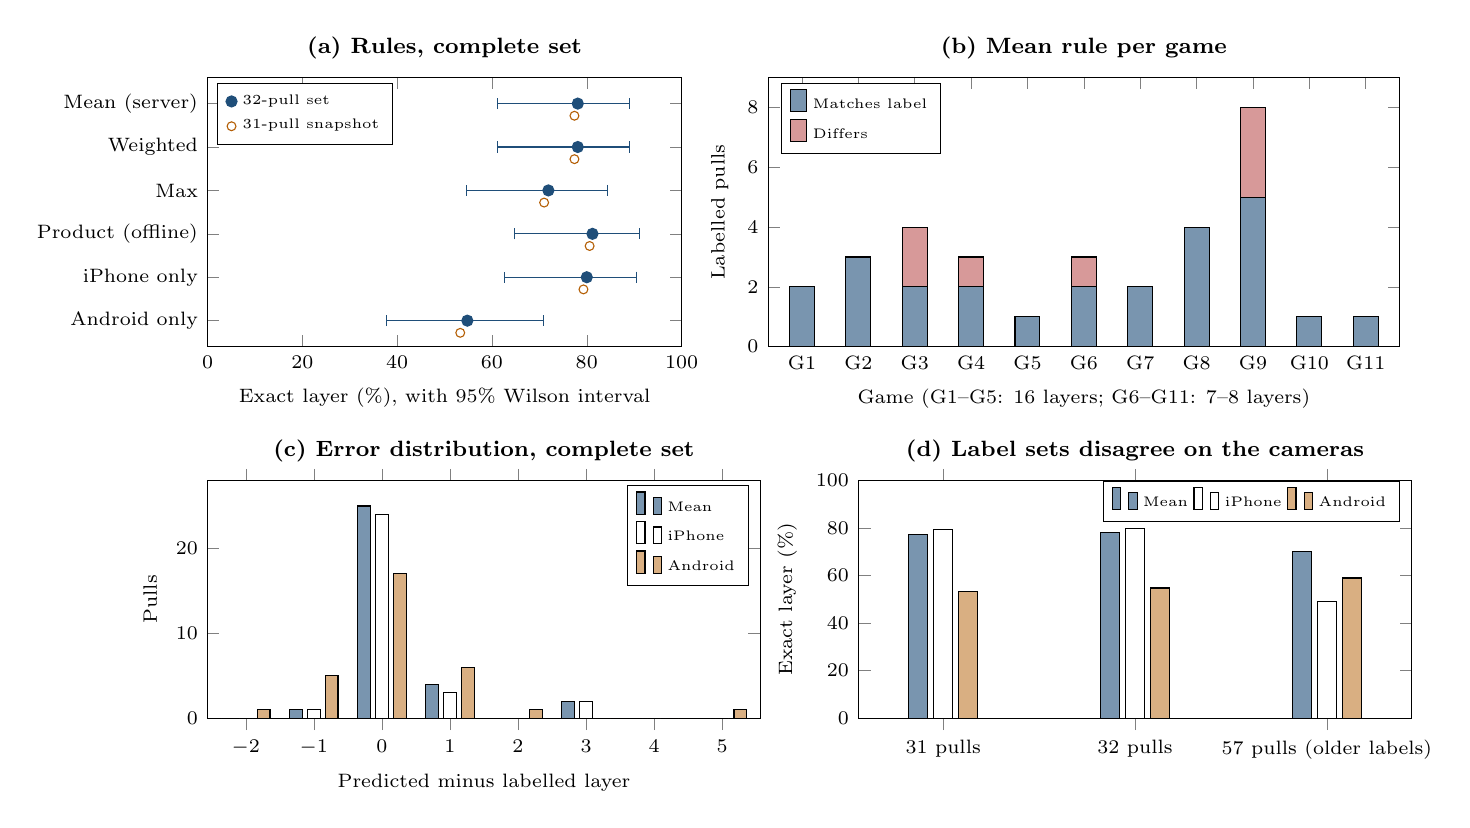
\begin{tikzpicture}
\begin{axis}[name=a,width=7.6cm,height=5.0cm,xmin=0,xmax=100,ymin=0.4,ymax=6.6,
  ytick={1,2,3,4,5,6},yticklabels={Android only,iPhone only,{Product (offline)},Max,Weighted,Mean (server)},
  xlabel={Exact layer (\%), with 95\% Wilson interval},tick label style={font=\scriptsize},label style={font=\scriptsize},
  title={\footnotesize\bfseries (a) Rules, complete set},title style={yshift=-1mm},legend style={font=\tiny,at={(0.02,0.98)},anchor=north west},legend cell align=left]
\addplot[only marks,mark=*,cdata,error bars/.cd,x dir=both,x explicit] coordinates {
 (54.8,1) += (16.0,0) -= (17.0,0)
 (80.0,2) += (10.5,0) -= (17.3,0)
 (81.2,3) += (9.9,0) -= (16.5,0)
 (71.9,4) += (12.5,0) -= (17.3,0)
 (78.1,5) += (10.9,0) -= (16.9,0)
 (78.1,6) += (10.9,0) -= (16.9,0)};
\addlegendentry{32-pull set}
\addplot[only marks,mark=o,cctl,mark size=1.6pt] coordinates {(53.3,0.72) (79.3,1.72) (80.6,2.72) (71.0,3.72) (77.4,4.72) (77.4,5.72)};
\addlegendentry{31-pull snapshot}
\end{axis}
\begin{axis}[name=b,at={(a.east)},anchor=west,xshift=1.1cm,width=9.6cm,height=5.0cm,ybar stacked,bar width=9pt,ymin=0,ymax=9,
  xtick={1,...,11},xticklabels={G1,G2,G3,G4,G5,G6,G7,G8,G9,G10,G11},
  ylabel={Labelled pulls},xlabel={Game (G1--G5: 16 layers; G6--G11: 7--8 layers)},tick label style={font=\scriptsize},label style={font=\scriptsize},
  title={\footnotesize\bfseries (b) Mean rule per game},title style={yshift=-1mm},legend style={font=\tiny,at={(0.02,0.98)},anchor=north west},legend cell align=left,enlarge x limits=0.06]
\addplot[fill=cdata!60,draw=black] coordinates {(1,2)(2,3)(3,2)(4,2)(5,1)(6,2)(7,2)(8,4)(9,5)(10,1)(11,1)};
\addlegendentry{Matches label}
\addplot[fill=chum!45,draw=black] coordinates {(1,0)(2,0)(3,2)(4,1)(5,0)(6,1)(7,0)(8,0)(9,3)(10,0)(11,0)};
\addlegendentry{Differs}
\end{axis}
\begin{axis}[name=c,at={(a.south west)},anchor=north west,yshift=-1.7cm,width=8.6cm,height=4.6cm,ybar,bar width=4.5pt,ymin=0,ymax=28,
  xtick={-2,-1,0,1,2,3,4,5},xlabel={Predicted minus labelled layer},ylabel={Pulls},tick label style={font=\scriptsize},label style={font=\scriptsize},
  title={\footnotesize\bfseries (c) Error distribution, complete set},title style={yshift=-1mm},legend style={font=\tiny,at={(0.98,0.98)},anchor=north east},legend cell align=left,enlarge x limits=0.08]
\addplot[fill=cdata!60,draw=black] coordinates {(-2,0)(-1,1)(0,25)(1,4)(2,0)(3,2)(4,0)(5,0)};\addlegendentry{Mean}
\addplot[fill=white,draw=black] coordinates {(-2,0)(-1,1)(0,24)(1,3)(2,0)(3,2)(4,0)(5,0)};\addlegendentry{iPhone}
\addplot[fill=cctl!50,draw=black] coordinates {(-2,1)(-1,5)(0,17)(1,6)(2,1)(3,0)(4,0)(5,1)};\addlegendentry{Android}
\end{axis}
\begin{axis}[name=d,at={(c.east)},anchor=west,xshift=1.25cm,width=8.6cm,height=4.6cm,ybar,bar width=7pt,ymin=0,ymax=100,
  symbolic x coords={31 pulls,32 pulls,57 pulls (older labels)},xtick=data,ylabel={Exact layer (\%)},tick label style={font=\scriptsize},label style={font=\scriptsize},
  title={\footnotesize\bfseries (d) Label sets disagree on the cameras},title style={yshift=-1mm},legend style={font=\tiny,at={(0.98,1.0)},anchor=north east,legend columns=3},legend cell align=left,enlarge x limits=0.22]
\addplot[fill=cdata!60,draw=black] coordinates {(31 pulls,77.4)(32 pulls,78.1)(57 pulls (older labels),70)};\addlegendentry{Mean}
\addplot[fill=white,draw=black] coordinates {(31 pulls,79.3)(32 pulls,80.0)(57 pulls (older labels),49)};\addlegendentry{iPhone}
\addplot[fill=cctl!50,draw=black] coordinates {(31 pulls,53.3)(32 pulls,54.8)(57 pulls (older labels),59)};\addlegendentry{Android}
\end{axis}
\end{tikzpicture}
\caption{Finder results, offline, with optimistic labels. (a) Rules with Wilson intervals, which assume independence; the product rule is exploratory. (b) Per-game outcomes, showing clustering. (c) Layer error. (d) iPhone and Android reverse between label sets; the cause is unresolved, and the 57-pull values are reported percentages.}\label{fig:finderplots}
\end{figure*}

\subsection{Pose and height: LiDAR versus baselines (RQ2)}
\emph{Pose} \evM\ (transcribed). Fig.~\ref{fig:poseheight}(a) and Table~\ref{tab:posedetail} show the comparison on 75 hand-free iPhone frames. The LiDAR fit did not improve the proxy (2.95 against 3.07 for markers alone; better on 41\,\% of frames). Snapping raised the score on every frame, but it optimises this same score, so this shows that the optimiser works and not that the overlay is more correct. Position error in millimetres was not measured. On five Android frames (E11), snapping moved the pose by at most 2.4\,mm and 0.8$^\circ$ and roughly doubled the score \evE.

The fitted corrections were also larger than expected: shifts of 4.9--12.8\,mm and tilts of 2.2--7.05$^\circ$ per run. Their cause is unexplained \evU. A partly visible tower might mislead the fit, and the largest may predate a board recalibration, but neither was tested.

\emph{Height} \evM\ (transcribed). On 233 hand-free frames from 3 towers, the 98th percentile of height got the exact layer on 98\,\% of frames, against 88\,\% for all box fits (Fig.~\ref{fig:poseheight}b), with mean bias $+0.02$ against $+0.10$ to $+0.13$ layers. The effective sample is closer to 3 towers than to 233 frames. The bias suggests that the fit reads slightly tall, which would explain the wrong layers. All methods were within one layer on every frame.

\emph{Synthetic stress.} With a hand simulated by replacing a share of near points (Fig.~\ref{fig:poseheight}c), box fits had lower height error than the percentile at every hand fraction tested, including 0.19 against 0.71 layers at 10\,\%. The robust schedule did not consistently beat plain least squares. So a box fit may help when a hand is in view, but only in synthetic data, and the server already skips depth frames while a hand is active.

\emph{Interpretation.} We distinguish four things. The \emph{intended purpose} of the LiDAR fit was a better overlay and height. The \emph{measured performance} shows no improvement over markers or a percentile on clean frames. \emph{Potential usefulness} remains for occluded frames and for telling the tower is standing without markers. The \emph{demonstrated improvement} in overlay accuracy is none.

\begin{figure*}[!t]\centering
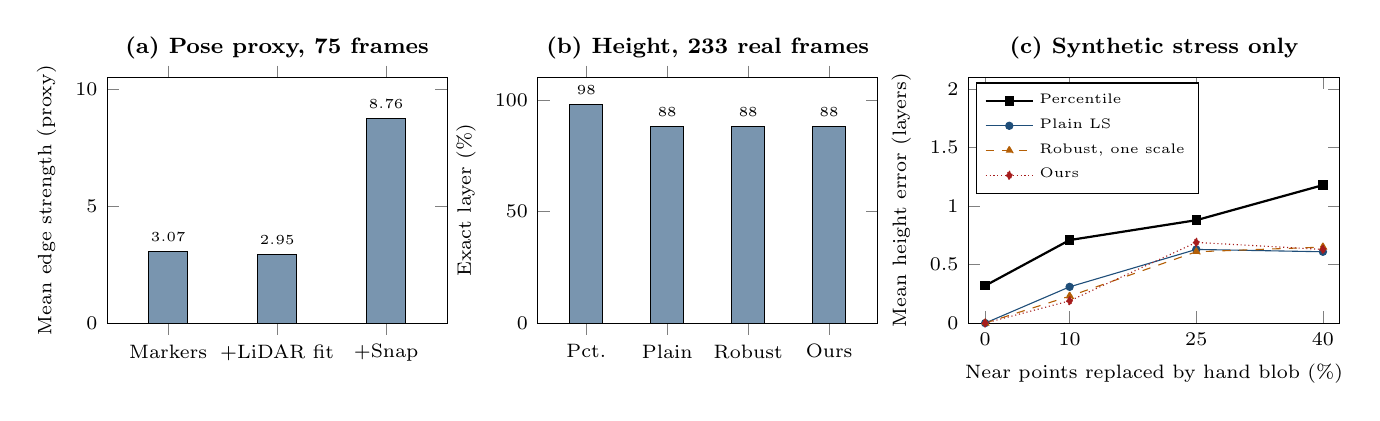
\begin{tikzpicture}
\begin{axis}[name=a,width=5.9cm,height=4.7cm,ybar,bar width=14pt,ymin=0,ymax=10.5,
  symbolic x coords={Markers,+LiDAR fit,+Snap},xtick=data,ylabel={Mean edge strength (proxy)},
  tick label style={font=\scriptsize},label style={font=\scriptsize},nodes near coords,every node near coord/.style={font=\tiny},
  title={\footnotesize\bfseries (a) Pose proxy, 75 frames},title style={yshift=-1mm},enlarge x limits=0.28]
\addplot[fill=cdata!60,draw=black] coordinates {(Markers,3.07)(+LiDAR fit,2.95)(+Snap,8.76)};
\end{axis}
\begin{axis}[name=b,at={(a.east)},anchor=west,xshift=1.15cm,width=5.9cm,height=4.7cm,ybar,bar width=12pt,ymin=0,ymax=110,
  symbolic x coords={Pct.,Plain,Robust,Ours},xtick=data,ylabel={Exact layer (\%)},
  tick label style={font=\scriptsize},label style={font=\scriptsize},nodes near coords,every node near coord/.style={font=\tiny},
  title={\footnotesize\bfseries (b) Height, 233 real frames},title style={yshift=-1mm},enlarge x limits=0.2]
\addplot[fill=cdata!60,draw=black] coordinates {(Pct.,98)(Plain,88)(Robust,88)(Ours,88)};
\end{axis}
\begin{axis}[name=c,at={(b.east)},anchor=west,xshift=1.15cm,width=6.3cm,height=4.7cm,xmin=-2,xmax=42,ymin=0,ymax=2.1,
  xtick={0,10,25,40},xlabel={Near points replaced by hand blob (\%)},ylabel={Mean height error (layers)},
  tick label style={font=\scriptsize},label style={font=\scriptsize},legend style={font=\tiny,at={(0.02,0.98)},anchor=north west},legend cell align=left,
  title={\footnotesize\bfseries (c) Synthetic stress only},title style={yshift=-1mm}]
\addplot[black,mark=square*,mark size=1.3pt,thick] coordinates {(0,0.32)(10,0.71)(25,0.88)(40,1.18)};\addlegendentry{Percentile}
\addplot[cdata,mark=*,mark size=1.3pt] coordinates {(0,0)(10,0.31)(25,0.63)(40,0.61)};\addlegendentry{Plain LS}
\addplot[cctl,dashed,mark=triangle*,mark size=1.5pt] coordinates {(0,0)(10,0.23)(25,0.61)(40,0.65)};\addlegendentry{Robust, one scale}
\addplot[chum,densely dotted,mark=diamond*,mark size=1.6pt] coordinates {(0,0)(10,0.19)(25,0.69)(40,0.63)};\addlegendentry{Ours}
\end{axis}
\end{tikzpicture}
\caption{LiDAR compared with simpler baselines; values are from transcribed terminal logs. (a) Edge-strength proxy: snapping optimises the same score, so its gain is circular. (b) Real, hand-free frames from 3 towers. (c) Synthetic 12-layer tower, 15 trials per level; not real data.}\label{fig:poseheight}
\end{figure*}

\begin{table}[!t]
\caption{Pose and height details, from transcribed logs of 2026-11-07.}\label{tab:posedetail}
\centering\footnotesize
\begin{tabular}{@{}p{3.15cm}rrr@{}}
\toprule
Run (layers), frames used & Shift (mm) & Tilt ($^\circ$) & Height frames \\
\midrule
20261102\_133032 (8) & 12.8 & 7.05 & 38 \\
20261106\_092828 (7) & 4.9 & 2.80 & 151 \\
20261106\_093055 (7) & 5.2 & 2.21 & 44 \\
\midrule
Height method & MAE & Bias & Time (ms) \\
\midrule
98th percentile & 0.02 & $+$0.02 & 1 \\
Box fit, plain LS & 0.12 & $+$0.10 & 51 \\
Box fit, robust, one scale & 0.13 & $+$0.13 & 51 \\
Box fit, schedule (ours) & 0.13 & $+$0.13 & about 55$^\dagger$ \\
\bottomrule
\end{tabular}

\vspace{2pt}{\footnotesize Shift is the vector norm of the logged correction. $^\dagger$The log records 2557\,ms, which the log's header calls a one-off slowdown; a separate re-timing gave about 55\,ms.}
\end{table}

\subsection{Collapse detection (RQ4)}
Table~\ref{tab:collapse} keeps the two collapse experiments apart. Under the current detector, the one real fall was declared 381\,s into its session (194 depth frames), and the two other sessions (66 and 99 depth frames) raised nothing. One detection has a Wilson interval of 21--100\,\%, so this does not validate the detector. Its guards were also designed on these and similar sessions, and the lens case was simulated by blanking depth (\code{COVER_S}), not tested with a real hand.

\begin{table}[!t]
\caption{Collapse experiments. They are not comparable and are not combined.}\label{tab:collapse}
\centering\footnotesize
\begin{tabular}{@{}p{1.4cm}p{2.85cm}p{3.5cm}@{}}
\toprule
 & Current detector (E12) & Older detector (E13) \\
\midrule
Date & Current code & 25 October \\
Method & Fit, height watch, standing check, guards & Height only \\
Data & 3 depth replays & 3 recorded collapses, 1 clean game \\
Result & 1 fall caught; 0 false alarms in 2 others & 3/3 caught; silent on the clean game \\
Use here & Current evidence & History only; superseded \\
\bottomrule
\end{tabular}
\end{table}

\subsection{Rule compiler (upstream)}
The stored upstream results \evM\ show 15 of 16 corpus entries compiling with a 120B-parameter hosted model and 7 of 16 with an 8B local model, and 4 of 80 claims in generated reports unsupported (5.0\,\%, Wilson 2--12\,\%). This code lives in another repository and was not re-run. It is included because it supplies the interface's rule layer; the Jenga legality overlay shown in this paper uses the balance rules in Section~\ref{sec:balance}.

\section{Qualitative Findings}\label{sec:qual}
Table~\ref{tab:failures} records the failure modes met during development. Causes are marked as tested only where evidence supports them. We highlight six themes.

\emph{Tracking when hands occlude.} Pose comes from the board rather than the tower, so the outline stays put while a hand is at the tower \evO. The price is reliance on the markers: small markers (below 28\,px) drop the overlay, and three visible markers can produce wrong poses unless many starts are tried.

\emph{Camera disagreement.} The Android view is lower and more oblique, which the team believes makes faces smaller and more occluded. That is a plausible explanation, not a tested one, particularly since label sets disagree on which camera is better. The system fuses scores without weighting.

\emph{Why simple baselines won.} The percentile is hard to beat on clean frames because the top of a standing tower is close to the highest points. The fit must explain partial views with a whole-box model, so small biases have room to appear. This is an interpretation consistent with the logged $+0.13$-layer bias.

\emph{Human interaction.} The system is built around a person. The player taps MARK, confirms or types the move, and can lock the overlay. Bondi et al.'s result~\cite{bondi2022} suggests a hypothesis we did not test: because the Yes/No prompt shows the finder's answer, it may anchor the player, and an unchallenged wrong answer would then enter the evaluation as correct. Tired or trusting players would have the same effect on labels.

\emph{Incorrect predictions.} Stored scores show errors of one layer more often than larger errors, which fits adjacent layers looking similar, but we cannot view the frames here to confirm a cause.

\emph{Silent failure paths.} Exceptions in depth handling are swallowed, and the pose is held for up to 6\,s without markers. Both keep the demo running and can hide faults.

\begin{table*}[!t]
\caption{Failure modes and their status. ``Cause'' is the team's explanation unless marked as tested.}\label{tab:failures}
\centering\footnotesize
\begin{tabular}{@{}p{3.0cm}p{4.1cm}p{4.2cm}p{3.1cm}p{1.8cm}@{}}
\toprule
Failure & What was seen & Cause & Response & Class \\
\midrule
Three markers visible & Solver could land on a wrong pose & Several poses fit three centres at a low angle & 24 seeded starts, corners decide & \evO \\
Board layout wrong & Overlay about 38\,mm off, frame tilted, on one board & Printed layout did not match the real sheet & LiDAR fit, board calibration & \evO \\
LiDAR correction on Android & Overlay one layer too high & Carried the iPhone's pose error to another camera & iPhone only & \evO \\
Hand over the lens & Looked like a fall & Could not tell covered lens from a fall & Lens guard, p95 corroboration; replay simulation only & \evU \\
Legal pulls fired the height watch & False game-over risk & Pulled blocks return to the top & Effective-tower flag; 9--22\,mm rise accepted & \evO \\
Fit read low after top pulls & 100\,mm reported on a 140\,mm tower & Partial top confuses fit & Second, p95 check must agree & \evO \\
Camera results disagree & Android better on 57 pulls, iPhone on 31 and 32 & Unknown; label sets differ & No device claim & \evU \\
Tall towers & 1/7, 9/9 and 10/13 under different conditions & Not established & Reported separately & \evU \\
Tracking pauses & Saved-frame gaps of 5.2 and 3.6\,s & Possibly limited tracking; not logged & App pauses saves & \evU \\
Loose block & Works on injected 5 and 8\,mm offsets & Never seen on a real loose block & Amber colour remains untested & \evU \\
\bottomrule
\end{tabular}
\end{table*}

\section{Discussion}\label{sec:discussion}
\textbf{RQ1.} The rig sustains about 3\,Hz saved frames at about 0.8\,MB each, and the decimation design explains the observed cadence. Wired benefit and end-to-end latency remain unknown.

\textbf{RQ2.} On available evidence, LiDAR did not earn its keep for overlay placement or clean-frame height. It remains useful as a sensor that works when markers are hidden, for telling the tower has fallen and for reading height without typing. Those benefits are observed or, for occlusion, synthetic. A negative result on a proxy is not proof that the fit is harmful, and the correct next step is to measure millimetre error against hand-clicked corners.

\textbf{RQ3.} The finder's scoring appears useful: about four in five exact and nearly all within one layer offline. That number needs its three qualifications together: offline conditions, optimistic labels, and few correlated games. Quantitative and qualitative evidence agree on one practical point: errors are mostly nearby and the player can catch them, so the design that keeps a human in the loop is justified for now. Claims about cameras and tall towers are not supported in either direction.

\textbf{RQ4.} The detector's guards each came from a real false alarm, which is a reasonable engineering process but tunes the detector on its own test data. The evidence supports ``worked on the few sessions we have'' and no more.

\textbf{RQ5.} The system is not autonomous. Below the gate, the player types the move; above it, the player confirms. Placements are assumed. Because labels depend on the same player, accuracy and human behaviour cannot be separated with the current data. As~\cite{bondi2022} argues for human-AI teams, the team should be evaluated as a team.

\textbf{System versus evaluation limits.} \emph{System limits}: fixed phones and a printed board, no observed placements, no multi-block detection unless the top drops, a straight-tower balance model with no friction, Android has no depth, and setup scripts assume a Mac. \emph{Evaluation limits}: optimistic labels, small clustered samples, in-sample tuning, offline approximations, missing logs, a proxy for pose, and data that others cannot inspect.

\section{Threats to Validity}\label{sec:threats}
We follow the aspects in~\cite{runeson2009} and add reproducibility. Table~\ref{tab:evidence} traces the main claims to their evidence.

\emph{Construct validity.} Edge strength is a proxy for overlay accuracy. ``Exact layer'' uses labels that count uncorrected confident answers as correct, which may inflate accuracy, hide confident errors, flatter tiers, and distort device comparisons if one camera drives the labelled answer. Frame differencing measures motion, not hands.

\emph{Internal validity.} Constants, tiers and guards were chosen on the data evaluated. The product rule was selected post hoc. Offline runs differ from the live path (Table~\ref{tab:offline}), and only typed-path moves are in the set. Replay with an uncorrected pose may explain the 1/7 result, but this is not established. The reason for the 57-pull disagreement and for the 32nd pull's earlier absence are both unknown.

\emph{External validity.} One tower, one board, one lighting setup, one iPhone model and players from the team. Nothing supports claims about other sets, rooms or players. As a case study, the work may generalise analytically, not statistically~\cite{runeson2009}.

\emph{Reliability.} Results depend on the authors' setup, and the authors labelled their own games. Stage timings came from a different machine with no original log. Benchmark logs are transcribed from a terminal. Each timing or benchmark ran once.

\emph{Reproducibility.} Code, stored finder scores and transcribed logs are public. Finder tallies can be recomputed from \code{variant_scores.json}. Recordings are private, so the benchmarks cannot be re-run by others, and \code{benchmark_height.py} currently fails with a missing \code{time} import. Replay tests need the same recordings.

\begin{table*}[!t]
\caption{Evidence traceability for the main claims.}\label{tab:evidence}
\centering\footnotesize
\begin{tabular}{@{}p{5.0cm}p{4.7cm}p{1.9cm}p{2.0cm}p{2.0cm}@{}}
\toprule
Claim & Source & Sample & Class & Provenance \\
\midrule
Mean rule: 25/32 exact offline & \code{variant_scores.json}, \code{eval_variants.py} & 32 pulls, 11 games & \evM & Stored, re-derived \\
Historical 24/31 is a subset without one game & Same, \code{RESULTS.md} & 31, 10 games & \evM & Re-derived \\
Product rule 26/32 & \code{eval_variants.py} only & 32 & \evE & Stored, re-derived \\
Weighted rule ties mean & Same & 32 & \evM & Stored, re-derived \\
iPhone versus Android inconclusive & \code{RESULTS.md}, stored scores & 29; 57 & \evU & Stored; reported \\
Fit not better than markers on proxy & \code{benchmark_pose.py}, its log & 75 frames & \evM & Transcribed \\
Percentile beats fit on clean frames & \code{benchmark_height.py}, its log & 233 frames & \evM & Transcribed \\
Current detector: one fall, no false alarm & Analysis files, earlier draft & 3 games & \evM & Reported \\
Lens guard works & \code{test_height_replay.py}, \code{COVER_S} & Simulation & \evU & Reported \\
Loose-block warning works on real blocks & \code{test_loose_replay.py} & Injected only & \evU & Reported \\
Hand gate is frame differencing & \code{tracker/iphone_saved.py} & Code & \evO & Source \\
Balance rule cases & \code{test_jenga_rules.py} & Unit tests & \evM & Re-run \\
\bottomrule
\end{tabular}
\end{table*}

\section{Conclusion}
Third Eye shows that a phone rig, a fixed marker board, explicit balance rules and a player in the loop can referee a Jenga game end to end, on one setup. Offline, the deployed scoring rule got 25 of 32 pulls exactly, with labels that favour it. The LiDAR box fit did not beat markers on an edge proxy or a percentile on clean height frames, and we report those as results rather than remove them. The current collapse detector has one real event behind it.

Future work \evP\ follows directly from these gaps: (i) a held-out test with frozen settings and independent ground truth, such as video review of each pull; (ii) overlay error in millimetres against hand-clicked corners; (iii) counts of each label type and a resolution of the 57-pull disagreement; (iv) logged MARK-to-answer time, wired-versus-Wi-Fi rate and stage timings; (v) more recorded falls, including a real hand over the lens and a real loose block; (vi) a measurement of how the Yes/No prompt affects players.

\section*{Acknowledgment}
% CONFIRM BEFORE SUBMISSION: check this disclosure against the current course and RV University AI policy.
AI-use disclosure: Claude (Anthropic) assisted with this manuscript's drafting and structure, its diagrams and tables, the recalculation of statistics from stored scores, and verification of references across all sections. An AI assistant also helped write parts of the project's code. Experiments were run by the authors, who are responsible for the accuracy and integrity of this paper.

\begin{thebibliography}{99}
\bibitem{fazeli2019} N.~Fazeli, M.~Oller, J.~Wu, Z.~Wu, J.~B. Tenenbaum, and A.~Rodriguez, ``See, feel, act: Hierarchical learning for complex manipulation skills with multisensory fusion,'' \emph{Science Robotics}, vol.~4, no.~26, art. eaav3123, 2019, doi: 10.1126/scirobotics.aav3123.
\bibitem{wolflein2021} G.~W\"olflein and O.~Arandjelovi\'c, ``Determining chess game state from an image,'' \emph{J. Imaging}, vol.~7, no.~6, art.~94, 2021, doi: 10.3390/jimaging7060094.
\bibitem{sener2022} F.~Sener, D.~Chatterjee, D.~Shelepov, K.~He, D.~Singhania, R.~Wang, and A.~Yao, ``Assembly101: A large-scale multi-view video dataset for understanding procedural activities,'' in \emph{Proc. IEEE/CVF CVPR}, 2022, pp. 21064--21074, doi: 10.1109/CVPR52688.2022.02042.
\bibitem{ding2023} G.~Ding, F.~Sener, S.~Ma, and A.~Yao, ``Every mistake counts in assembly,'' arXiv:2307.16453, 2023.
\bibitem{wang2016} X.~Wang, S.~K. Ong, and A.~Y.~C. Nee, ``A comprehensive survey of augmented reality assembly research,'' \emph{Advances in Manufacturing}, vol.~4, no.~1, pp. 1--22, 2016, doi: 10.1007/s40436-015-0131-4.
\bibitem{garrido2014} S.~Garrido-Jurado, R.~Mu\~noz-Salinas, F.~J. Madrid-Cuevas, and M.~J. Mar\'in-Jim\'enez, ``Automatic generation and detection of highly reliable fiducial markers under occlusion,'' \emph{Pattern Recognition}, vol.~47, no.~6, pp. 2280--2292, 2014, doi: 10.1016/j.patcog.2014.01.005.
\bibitem{collins2014} T.~Collins and A.~Bartoli, ``Infinitesimal plane-based pose estimation,'' \emph{Int. J. Comput. Vis.}, vol.~109, no.~3, pp. 252--286, 2014, doi: 10.1007/s11263-014-0725-5.
\bibitem{triggs2000} B.~Triggs, P.~F. McLauchlan, R.~I. Hartley, and A.~W. Fitzgibbon, ``Bundle adjustment---A modern synthesis,'' in \emph{Vision Algorithms: Theory and Practice}, LNCS, vol.~1883. Springer, 2000, pp. 298--372, doi: 10.1007/3-540-44480-7\_21.
\bibitem{zhang2000} Z.~Zhang, ``A flexible new technique for camera calibration,'' \emph{IEEE Trans. Pattern Anal. Mach. Intell.}, vol.~22, no.~11, pp. 1330--1334, 2000, doi: 10.1109/34.888718.
\bibitem{drummond2002} T.~Drummond and R.~Cipolla, ``Real-time visual tracking of complex structures,'' \emph{IEEE Trans. Pattern Anal. Mach. Intell.}, vol.~24, no.~7, pp. 932--946, 2002, doi: 10.1109/TPAMI.2002.1017620.
\bibitem{luetzenburg2021} G.~Luetzenburg, A.~Kroon, and A.~A. Bj{\o}rk, ``Evaluation of the Apple iPhone 12 Pro LiDAR for an application in geosciences,'' \emph{Scientific Reports}, vol.~11, 2021, doi: 10.1038/s41598-021-01763-9.
\bibitem{huang2023} Z.~Huang, K.~Yao, S.~Z. Zhao, C.~Pan, and A.~Y. Yang, ``Robust 6DoF pose estimation against depth noise and a comprehensive evaluation on a mobile dataset,'' arXiv:2309.13570v5, 2025.
\bibitem{newcombe2011} R.~A. Newcombe \emph{et al.}, ``KinectFusion: Real-time dense surface mapping and tracking,'' in \emph{Proc. IEEE ISMAR}, 2011, pp. 127--136, doi: 10.1109/ISMAR.2011.6092378.
\bibitem{black1996} M.~J. Black and A.~Rangarajan, ``On the unification of line processes, outlier rejection, and robust statistics with applications in early vision,'' \emph{Int. J. Comput. Vis.}, vol.~19, no.~1, pp. 57--91, 1996, doi: 10.1007/BF00131148.
\bibitem{yang2020} H.~Yang, P.~Antonante, V.~Tzoumas, and L.~Carlone, ``Graduated non-convexity for robust spatial perception: From non-minimal solvers to global outlier rejection,'' \emph{IEEE Robot. Autom. Lett.}, vol.~5, no.~2, pp. 1127--1134, 2020, doi: 10.1109/LRA.2020.2965893.
\bibitem{radke2005} R.~J. Radke, S.~Andra, O.~Al-Kofahi, and B.~Roysam, ``Image change detection algorithms: A systematic survey,'' \emph{IEEE Trans. Image Process.}, vol.~14, no.~3, pp. 294--307, 2005, doi: 10.1109/TIP.2004.838698.
\bibitem{kuglin1975} C.~D. Kuglin and D.~C. Hines, ``The phase correlation image alignment method,'' in \emph{Proc. IEEE Int. Conf. Cybernetics and Society}, 1975, pp. 163--165.
\bibitem{chow1970} C.~K. Chow, ``On optimum recognition error and reject tradeoff,'' \emph{IEEE Trans. Inf. Theory}, vol.~16, no.~1, pp. 41--46, 1970, doi: 10.1109/TIT.1970.1054406.
\bibitem{guo2017} C.~Guo, G.~Pleiss, Y.~Sun, and K.~Q. Weinberger, ``On calibration of modern neural networks,'' in \emph{Proc. ICML}, PMLR, vol.~70, 2017, pp. 1321--1330.
\bibitem{bondi2022} E.~Bondi, R.~Koster, H.~Sheahan, M.~Chadwick, Y.~Bachrach, T.~Cemgil, U.~Paquet, and K.~Dvijotham, ``Role of human-AI interaction in selective prediction,'' in \emph{Proc. AAAI}, vol.~36, no.~5, 2022, pp. 5286--5294, doi: 10.1609/aaai.v36i5.20465.
\bibitem{mensfelt2025} A.~Mensfelt, K.~Stathis, and V.~Trencsenyi, ``Generative agents for multi-agent autoformalization of interaction scenarios,'' arXiv:2412.08805v3, 2025.
\bibitem{runeson2009} P.~Runeson and M.~H\"ost, ``Guidelines for conducting and reporting case study research in software engineering,'' \emph{Empirical Softw. Eng.}, vol.~14, no.~2, pp. 131--164, 2009, doi: 10.1007/s10664-008-9102-8.
\bibitem{wilson1927} E.~B. Wilson, ``Probable inference, the law of succession, and statistical inference,'' \emph{J. Amer. Statist. Assoc.}, vol.~22, no.~158, pp. 209--212, 1927, doi: 10.1080/01621459.1927.10502953.
\bibitem{agresti1998} A.~Agresti and B.~A. Coull, ``Approximate is better than `exact' for interval estimation of binomial proportions,'' \emph{Amer. Statistician}, vol.~52, no.~2, pp. 119--126, 1998, doi: 10.1080/00031305.1998.10480550.
\bibitem{brown2001} L.~D. Brown, T.~T. Cai, and A.~DasGupta, ``Interval estimation for a binomial proportion,'' \emph{Statist. Sci.}, vol.~16, no.~2, pp. 101--133, 2001, doi: 10.1214/ss/1009213286.
\bibitem{field2007} C.~A. Field and A.~H. Welsh, ``Bootstrapping clustered data,'' \emph{J. R. Stat. Soc. Ser. B}, vol.~69, no.~3, pp. 369--390, 2007, doi: 10.1111/j.1467-9868.2007.00593.x.
\end{thebibliography}
\end{document}
